% Options for packages loaded elsewhere
\PassOptionsToPackage{unicode}{hyperref}
\PassOptionsToPackage{hyphens}{url}
\PassOptionsToPackage{dvipsnames,svgnames,x11names}{xcolor}
%
\documentclass[
  11pt,
]{article}

\usepackage{amsmath,amssymb}
\usepackage{iftex}
\ifPDFTeX
  \usepackage[T1]{fontenc}
  \usepackage[utf8]{inputenc}
  \usepackage{textcomp} % provide euro and other symbols
\else % if luatex or xetex
  \usepackage{unicode-math}
  \defaultfontfeatures{Scale=MatchLowercase}
  \defaultfontfeatures[\rmfamily]{Ligatures=TeX,Scale=1}
\fi
\usepackage{lmodern}
\ifPDFTeX\else  
    % xetex/luatex font selection
\fi
% Use upquote if available, for straight quotes in verbatim environments
\IfFileExists{upquote.sty}{\usepackage{upquote}}{}
\IfFileExists{microtype.sty}{% use microtype if available
  \usepackage[]{microtype}
  \UseMicrotypeSet[protrusion]{basicmath} % disable protrusion for tt fonts
}{}
\makeatletter
\@ifundefined{KOMAClassName}{% if non-KOMA class
  \IfFileExists{parskip.sty}{%
    \usepackage{parskip}
  }{% else
    \setlength{\parindent}{0pt}
    \setlength{\parskip}{6pt plus 2pt minus 1pt}}
}{% if KOMA class
  \KOMAoptions{parskip=half}}
\makeatother
\usepackage{xcolor}
\usepackage[margin=1in]{geometry}
\setlength{\emergencystretch}{3em} % prevent overfull lines
\setcounter{secnumdepth}{-\maxdimen} % remove section numbering
% Make \paragraph and \subparagraph free-standing
\ifx\paragraph\undefined\else
  \let\oldparagraph\paragraph
  \renewcommand{\paragraph}[1]{\oldparagraph{#1}\mbox{}}
\fi
\ifx\subparagraph\undefined\else
  \let\oldsubparagraph\subparagraph
  \renewcommand{\subparagraph}[1]{\oldsubparagraph{#1}\mbox{}}
\fi

\usepackage{color}
\usepackage{fancyvrb}
\newcommand{\VerbBar}{|}
\newcommand{\VERB}{\Verb[commandchars=\\\{\}]}
\DefineVerbatimEnvironment{Highlighting}{Verbatim}{commandchars=\\\{\}}
% Add ',fontsize=\small' for more characters per line
\usepackage{framed}
\definecolor{shadecolor}{RGB}{241,243,245}
\newenvironment{Shaded}{\begin{snugshade}}{\end{snugshade}}
\newcommand{\AlertTok}[1]{\textcolor[rgb]{0.68,0.00,0.00}{#1}}
\newcommand{\AnnotationTok}[1]{\textcolor[rgb]{0.37,0.37,0.37}{#1}}
\newcommand{\AttributeTok}[1]{\textcolor[rgb]{0.40,0.45,0.13}{#1}}
\newcommand{\BaseNTok}[1]{\textcolor[rgb]{0.68,0.00,0.00}{#1}}
\newcommand{\BuiltInTok}[1]{\textcolor[rgb]{0.00,0.23,0.31}{#1}}
\newcommand{\CharTok}[1]{\textcolor[rgb]{0.13,0.47,0.30}{#1}}
\newcommand{\CommentTok}[1]{\textcolor[rgb]{0.37,0.37,0.37}{#1}}
\newcommand{\CommentVarTok}[1]{\textcolor[rgb]{0.37,0.37,0.37}{\textit{#1}}}
\newcommand{\ConstantTok}[1]{\textcolor[rgb]{0.56,0.35,0.01}{#1}}
\newcommand{\ControlFlowTok}[1]{\textcolor[rgb]{0.00,0.23,0.31}{#1}}
\newcommand{\DataTypeTok}[1]{\textcolor[rgb]{0.68,0.00,0.00}{#1}}
\newcommand{\DecValTok}[1]{\textcolor[rgb]{0.68,0.00,0.00}{#1}}
\newcommand{\DocumentationTok}[1]{\textcolor[rgb]{0.37,0.37,0.37}{\textit{#1}}}
\newcommand{\ErrorTok}[1]{\textcolor[rgb]{0.68,0.00,0.00}{#1}}
\newcommand{\ExtensionTok}[1]{\textcolor[rgb]{0.00,0.23,0.31}{#1}}
\newcommand{\FloatTok}[1]{\textcolor[rgb]{0.68,0.00,0.00}{#1}}
\newcommand{\FunctionTok}[1]{\textcolor[rgb]{0.28,0.35,0.67}{#1}}
\newcommand{\ImportTok}[1]{\textcolor[rgb]{0.00,0.46,0.62}{#1}}
\newcommand{\InformationTok}[1]{\textcolor[rgb]{0.37,0.37,0.37}{#1}}
\newcommand{\KeywordTok}[1]{\textcolor[rgb]{0.00,0.23,0.31}{#1}}
\newcommand{\NormalTok}[1]{\textcolor[rgb]{0.00,0.23,0.31}{#1}}
\newcommand{\OperatorTok}[1]{\textcolor[rgb]{0.37,0.37,0.37}{#1}}
\newcommand{\OtherTok}[1]{\textcolor[rgb]{0.00,0.23,0.31}{#1}}
\newcommand{\PreprocessorTok}[1]{\textcolor[rgb]{0.68,0.00,0.00}{#1}}
\newcommand{\RegionMarkerTok}[1]{\textcolor[rgb]{0.00,0.23,0.31}{#1}}
\newcommand{\SpecialCharTok}[1]{\textcolor[rgb]{0.37,0.37,0.37}{#1}}
\newcommand{\SpecialStringTok}[1]{\textcolor[rgb]{0.13,0.47,0.30}{#1}}
\newcommand{\StringTok}[1]{\textcolor[rgb]{0.13,0.47,0.30}{#1}}
\newcommand{\VariableTok}[1]{\textcolor[rgb]{0.07,0.07,0.07}{#1}}
\newcommand{\VerbatimStringTok}[1]{\textcolor[rgb]{0.13,0.47,0.30}{#1}}
\newcommand{\WarningTok}[1]{\textcolor[rgb]{0.37,0.37,0.37}{\textit{#1}}}

\providecommand{\tightlist}{%
  \setlength{\itemsep}{0pt}\setlength{\parskip}{0pt}}\usepackage{longtable,booktabs,array}
\usepackage{calc} % for calculating minipage widths
% Correct order of tables after \paragraph or \subparagraph
\usepackage{etoolbox}
\makeatletter
\patchcmd\longtable{\par}{\if@noskipsec\mbox{}\fi\par}{}{}
\makeatother
% Allow footnotes in longtable head/foot
\IfFileExists{footnotehyper.sty}{\usepackage{footnotehyper}}{\usepackage{footnote}}
\makesavenoteenv{longtable}
\usepackage{graphicx}
\makeatletter
\def\maxwidth{\ifdim\Gin@nat@width>\linewidth\linewidth\else\Gin@nat@width\fi}
\def\maxheight{\ifdim\Gin@nat@height>\textheight\textheight\else\Gin@nat@height\fi}
\makeatother
% Scale images if necessary, so that they will not overflow the page
% margins by default, and it is still possible to overwrite the defaults
% using explicit options in \includegraphics[width, height, ...]{}
\setkeys{Gin}{width=\maxwidth,height=\maxheight,keepaspectratio}
% Set default figure placement to htbp
\makeatletter
\def\fps@figure{htbp}
\makeatother

\usepackage[noblocks]{authblk}
\renewcommand*{\Authsep}{, }
\renewcommand*{\Authand}{, }
\renewcommand*{\Authands}{, }
\renewcommand\Affilfont{\small}
\makeatletter
\makeatother
\makeatletter
\makeatother
\makeatletter
\@ifpackageloaded{caption}{}{\usepackage{caption}}
\AtBeginDocument{%
\ifdefined\contentsname
  \renewcommand*\contentsname{Table of contents}
\else
  \newcommand\contentsname{Table of contents}
\fi
\ifdefined\listfigurename
  \renewcommand*\listfigurename{List of Figures}
\else
  \newcommand\listfigurename{List of Figures}
\fi
\ifdefined\listtablename
  \renewcommand*\listtablename{List of Tables}
\else
  \newcommand\listtablename{List of Tables}
\fi
\ifdefined\figurename
  \renewcommand*\figurename{Figure}
\else
  \newcommand\figurename{Figure}
\fi
\ifdefined\tablename
  \renewcommand*\tablename{Table}
\else
  \newcommand\tablename{Table}
\fi
}
\@ifpackageloaded{float}{}{\usepackage{float}}
\floatstyle{ruled}
\@ifundefined{c@chapter}{\newfloat{codelisting}{h}{lop}}{\newfloat{codelisting}{h}{lop}[chapter]}
\floatname{codelisting}{Listing}
\newcommand*\listoflistings{\listof{codelisting}{List of Listings}}
\makeatother
\makeatletter
\@ifpackageloaded{caption}{}{\usepackage{caption}}
\@ifpackageloaded{subcaption}{}{\usepackage{subcaption}}
\makeatother
\makeatletter
\@ifpackageloaded{tcolorbox}{}{\usepackage[skins,breakable]{tcolorbox}}
\makeatother
\makeatletter
\@ifundefined{shadecolor}{\definecolor{shadecolor}{rgb}{.97, .97, .97}}
\makeatother
\makeatletter
\makeatother
\makeatletter
\makeatother
\ifLuaTeX
  \usepackage{selnolig}  % disable illegal ligatures
\fi
\IfFileExists{bookmark.sty}{\usepackage{bookmark}}{\usepackage{hyperref}}
\IfFileExists{xurl.sty}{\usepackage{xurl}}{} % add URL line breaks if available
\urlstyle{same} % disable monospaced font for URLs
\hypersetup{
  pdftitle={Data Visualization Platform Report},
  pdfauthor={Yiqing Hu; Ting Wei; Xinchen Yang; Ludi Feng},
  colorlinks=true,
  linkcolor={blue},
  filecolor={Maroon},
  citecolor={Blue},
  urlcolor={Blue},
  pdfcreator={LaTeX via pandoc}}

\title{Data Visualization Platform Report}


\author[1]{Yiqing Hu}
\author[1]{Ting Wei}
\author[1]{Xinchen Yang}
\author[1]{Ludi Feng}

\affil[1]{University of Warsaw, Faculty of Economics Sciences}


\date{}
\begin{document}
\maketitle
\ifdefined\Shaded\renewenvironment{Shaded}{\begin{tcolorbox}[frame hidden, interior hidden, boxrule=0pt, sharp corners, borderline west={3pt}{0pt}{shadecolor}, breakable, enhanced]}{\end{tcolorbox}}\fi

\hypertarget{project-introduction}{%
\section{PROJECT INTRODUCTION}\label{project-introduction}}

The goal of this project was to create a dashboard application for an
e-commerce company's marketing, product development, and sales teams.
The application utilizes customer data to provide insights for
developing products and marketing plans targeted towards improving
customer engagement and sales.

The project used an e-commerce dataset, which contained information
about customer behavior data, purchase history, product preferences,
customer segmentation, and future forcasting of order and consumer.

Data preprocessing steps were outlined, including data cleaning and user
interface design using shinydashboard. The server function was
described, highlighting the filtering of data and creation of reactive
datasets. The report also mentioned the use of info boxes and graphs in
the dashboard.

Overall, the project created a dashboard application that presented
e-commerce data in a visually informative way, helping marketing,
product development, and sales teams make data-driven decisions.

\hypertarget{approch-method-used}{%
\section{APPROCH / METHOD USED}\label{approch-method-used}}

\hypertarget{writing-own-advanced-functions-in-r}{%
\subsection{Writing own advanced functions in
R}\label{writing-own-advanced-functions-in-r}}

Based on our specific requirements for data visualization, define the
function you want to create. Consider the parameters the function should
accept, such as the input data, visualization type, customization
options, or filters. In order to visualize e-commerce data within the
platform. Provide the necessary inputs and parameters to generate the
desired visualizations based on the function's capabilities.

\hypertarget{object-oriented-programming}{%
\subsection{Object-oriented
programming}\label{object-oriented-programming}}

Create instances of the defined classes as needed within the e-commerce
data visualization platform. Also implement some method based on the
object-oriented programming

\hypertarget{using-of-c-in-r}{%
\subsection{Using of C++ in R}\label{using-of-c-in-r}}

We will use Rcpp to interface with C++ code for computationally
intensive tasks. This will enable us to take advantage of the speed and
memory efficiency of C++ for critical parts of our application.

We achieve an C++ implementation of the K-means clustering algorithm
using the Rcpp library to integrate with R and perform the clustering
using the kmeans function from the ``stats'' package.

\hypertarget{vectorisation-of-the-code}{%
\subsection{Vectorisation of the code}\label{vectorisation-of-the-code}}

Using vectorization techniques to optimize our code and make it more
efficient. This will help us process large datasets quickly and
accurately, and enhance the user experience.

We will have a dataset of customer transactions with timestamps, and we
want to calculate the number of transactions that occurred within each
hour of the day. Instead of using explicit loops, we can leverage
vectorization techniques in R to perform this calculation efficiently.

By utilizing vectorization, we eliminate the need for explicit loops and
perform the calculation efficiently using built-in functions. This
approach is particularly useful when dealing with large datasets or
performing repetitive calculations.

Similarly, we can apply vectorization techniques to other scenarios in
our project, such as calculating statistics or performing aggregations
based on specific time intervals or other criteria.

By leveraging vectorization, we can process data efficiently and perform
calculations on large datasets in a concise and optimized manner,
leading to improved performance and overall efficiency in our project

\hypertarget{shiny-creating-analytical-dashboards}{%
\subsection{Shiny + creating analytical
dashboards}\label{shiny-creating-analytical-dashboards}}

We will leverage Shiny to create interactive and responsive dashboards
that enable users to explore and visualize data, and make informed
decisions. These dashboards will be user-friendly, intuitive, and
aesthetically pleasing.

\hypertarget{creating-own-r-packages}{%
\subsection{Creating own R packages}\label{creating-own-r-packages}}

We will create our own R package to encapsulate the functionality we
have developed. This package includes the generation of time series
data. As long as the original data has a basic time format, new time
series can be generated, including the year, quarter, month, week, and
day, and model training of different dimensions based on the newly
generated data. and forecast. Thus the new package will be data
compatible, modular, reusable and easy to maintain. We will also
leverage existing packages such as tidyverse, machine learning
techniques or time series/spatial data analysis to enhance our new
packages.

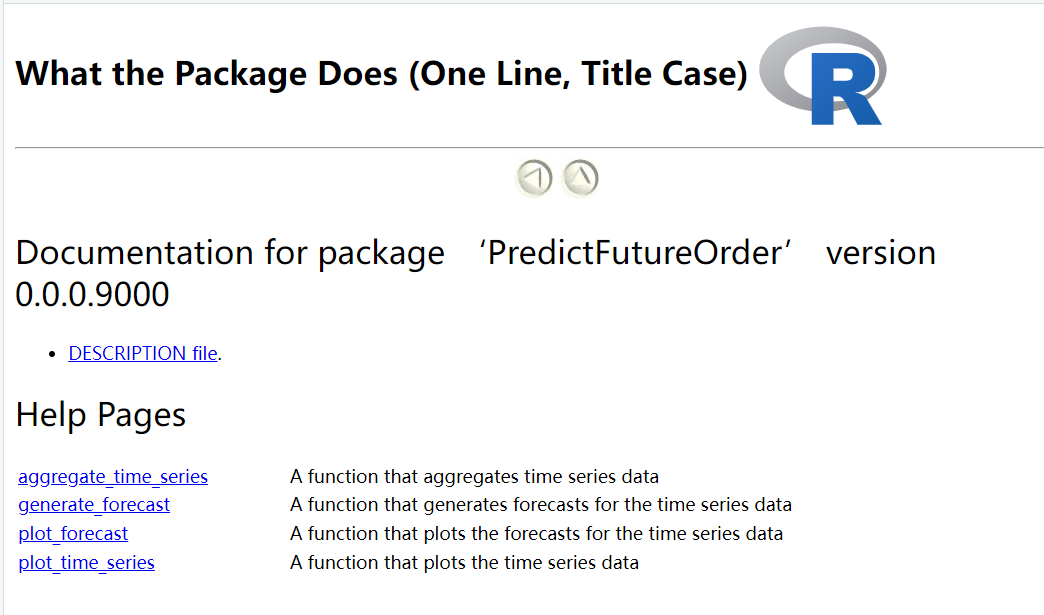
\includegraphics{img/R_pkg.png}

\begin{itemize}
\tightlist
\item
  aggregate\_time\_series
\end{itemize}

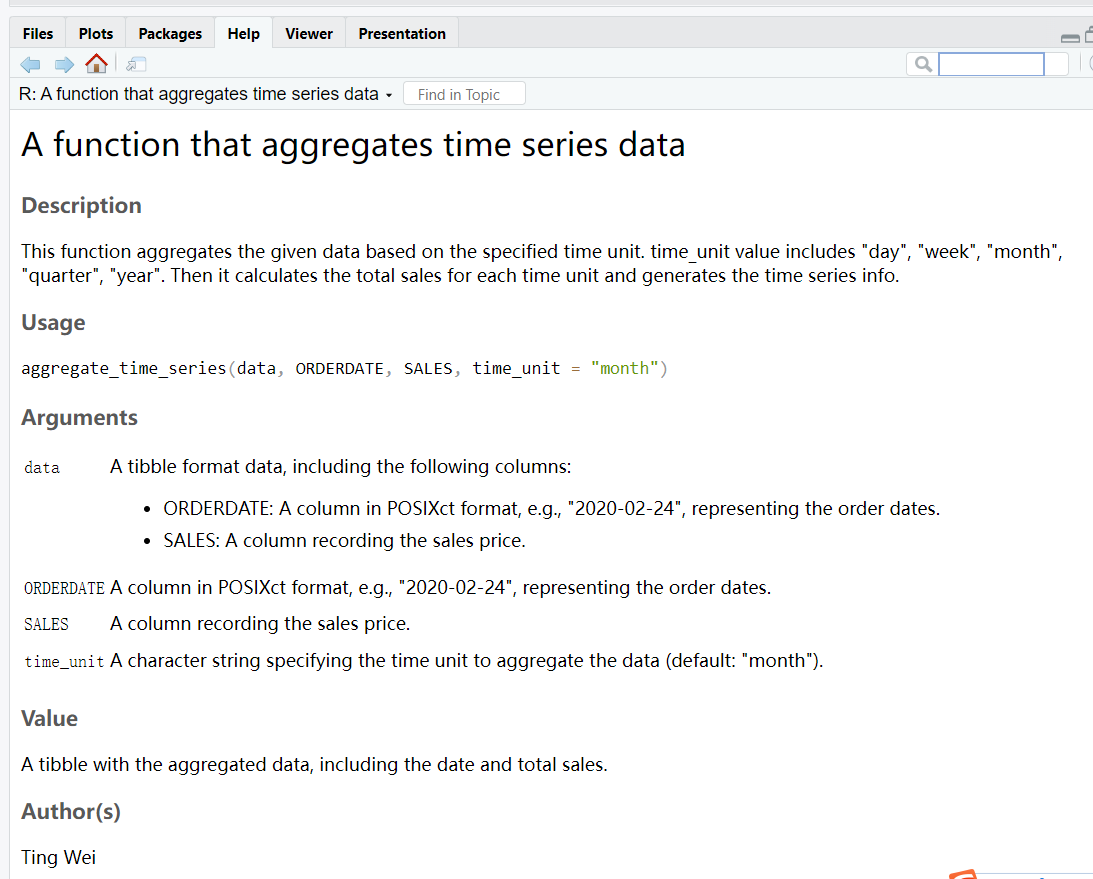
\includegraphics{img/aggregate_time_series.png}

\begin{itemize}
\tightlist
\item
  generate\_forecast
\end{itemize}

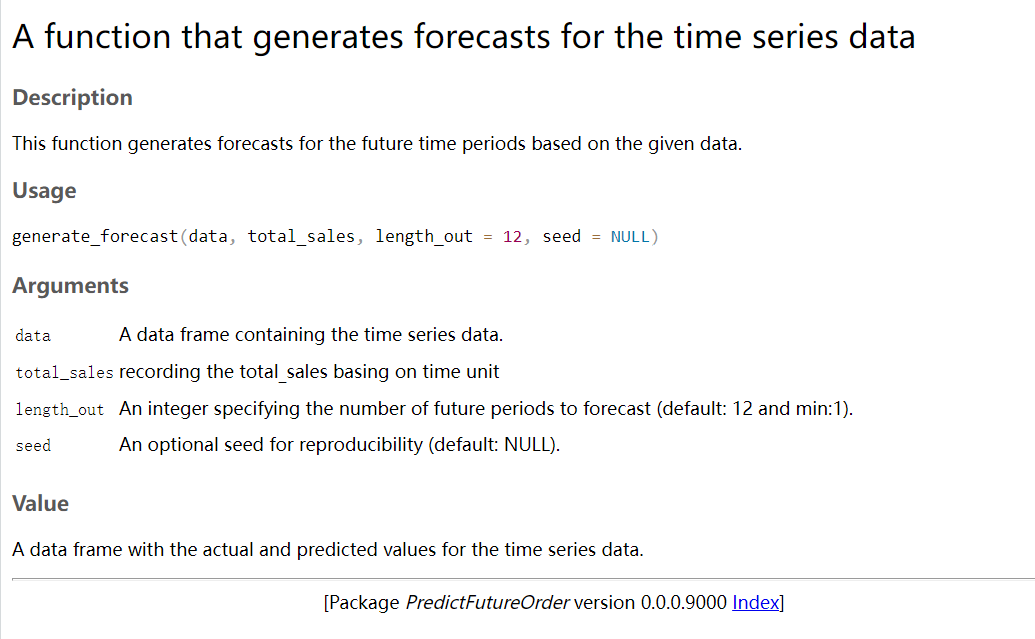
\includegraphics{img/generate_forecast.png}

\begin{itemize}
\tightlist
\item
  plot\_forecast
\end{itemize}

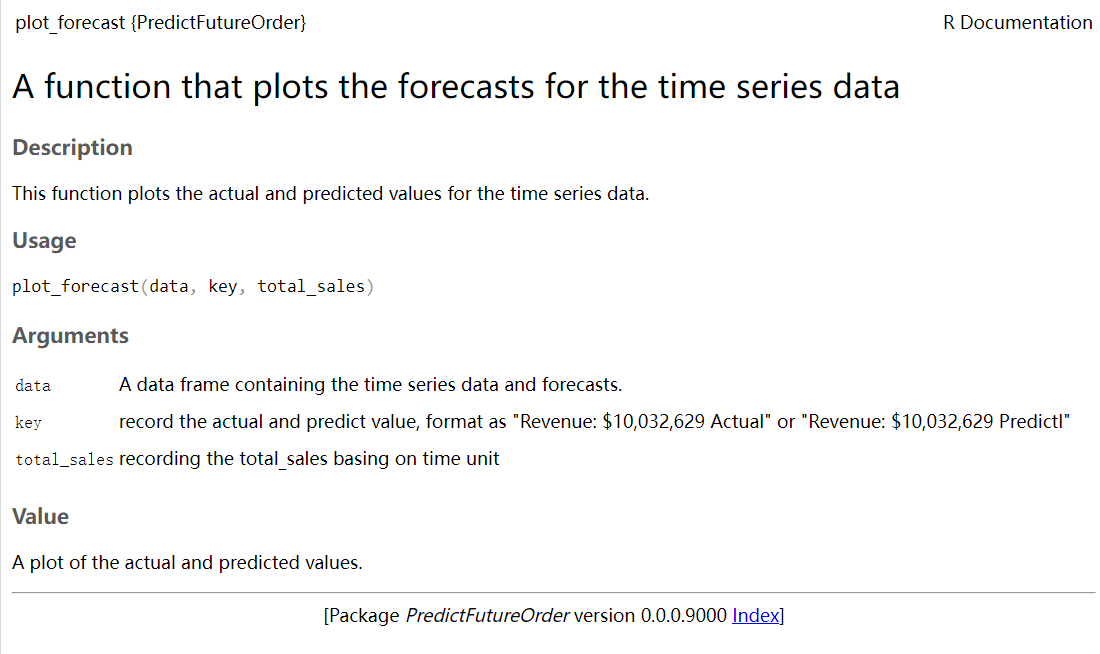
\includegraphics{img/plot_forecast.png}

\begin{itemize}
\tightlist
\item
  plot\_time\_series
\end{itemize}

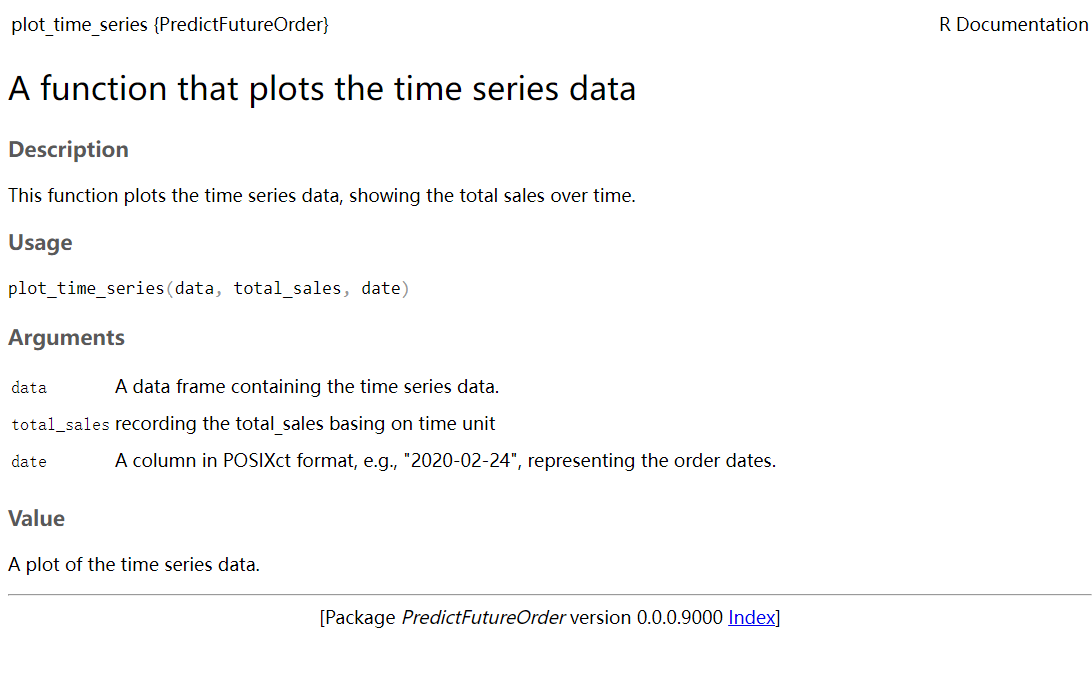
\includegraphics{img/plot_time_series.png}

\hypertarget{platforms-structure}{%
\section{PLATFORMS STRUCTURE}\label{platforms-structure}}

Using the shinydashboard package in R. which sets up a dashboard with a
header, sidebar, and main panel, and defines different tabs for each
page. In the platform, there are six tabs:

\begin{itemize}
\item
  ``Customer Activity Analysis'': This tab includes visualizations and
  analysis related to customer activity. Such as website visits, clicks,
  or logins, over a certain period.
\item
  ``Customer Order Analysis'': This tab focus on analyzing customer
  orders. Such as the total number of orders, revenue generated, the
  most popular products purchased, order trends over time.
\item
  ``Conversion Rate'': This tab could be dedicated to analyzing
  conversion rates, which refer to the percentage of users who complete
  a desired action (e.g., making a purchase) out of the total number of
  users who visit a specific page or take a specific action.
\item
  ``Consumer Segmentation'': This tab involves segmenting customers
  based on specific characteristics or behaviors. Such as high-value
  customers, frequent buyers, or lost customer.
\item
  ``Future Order Forecasting'': This tab focus on predicting future
  orders or sales. Using time series forecasting techniques and machine
  learning algorithms to generate forecasts based on historical data.
\item
  ``Customer Forecasting'': This tab is dedicated to forecasting
  customer-related metrics, such as customer classification trend, and
  customer lifetime value. Similar to the previous tab, using predictive
  modeling techniques to generate forecasts for these metrics.
\end{itemize}

\begin{Shaded}
\begin{Highlighting}[]
\NormalTok{ui }\OtherTok{\textless{}{-}} \FunctionTok{dashboardPage}\NormalTok{(}
  \FunctionTok{dashboardHeader}\NormalTok{(}\AttributeTok{title =} \StringTok{"Customer Dashboard"}\NormalTok{),}
  \FunctionTok{dashboardSidebar}\NormalTok{(}
    \FunctionTok{sidebarMenu}\NormalTok{( }\AttributeTok{width =} \DecValTok{160}\NormalTok{,}
      \AttributeTok{id =} \StringTok{"sidebar"}\NormalTok{,}
      \FunctionTok{menuItem}\NormalTok{(}\StringTok{"Customer Activity Analysis{-}HJ"}\NormalTok{, }\AttributeTok{tabName =} \StringTok{"page1"}\NormalTok{),}
      \FunctionTok{menuItem}\NormalTok{(}\StringTok{"Customer Order Analysis{-}HJ"}\NormalTok{, }\AttributeTok{tabName =} \StringTok{"page2"}\NormalTok{),}
      \FunctionTok{menuItem}\NormalTok{(}\StringTok{"Conversion Rate{-}YXC"}\NormalTok{, }\AttributeTok{tabName =} \StringTok{"page3"}\NormalTok{),}
      \FunctionTok{menuItem}\NormalTok{(}\StringTok{"Consumer Segmentation{-}YXC"}\NormalTok{, }\AttributeTok{tabName =} \StringTok{"page4"}\NormalTok{),}
      \FunctionTok{menuItem}\NormalTok{(}\StringTok{"Future Order Forecasting{-}WT"}\NormalTok{, }\AttributeTok{tabName =} \StringTok{"page5"}\NormalTok{),}
      \FunctionTok{menuItem}\NormalTok{(}\StringTok{"Customer Forecasting{-}WT"}\NormalTok{, }\AttributeTok{tabName =} \StringTok{"page6"}\NormalTok{)}
\NormalTok{    )}
\NormalTok{  ),}
  \FunctionTok{dashboardBody}\NormalTok{(}
    \FunctionTok{tabItems}\NormalTok{(}
      \CommentTok{\# Page 1}
      \FunctionTok{tabItem}\NormalTok{(}
        \AttributeTok{tabName =} \StringTok{"page1"}\NormalTok{,}
        \FunctionTok{sidebarLayout}\NormalTok{(}
          \FunctionTok{sidebarPanel}\NormalTok{(}
            \CommentTok{\# Add sidebar content for page 1 here}
            \FunctionTok{selectInput}\NormalTok{(}\StringTok{"page1\_filter"}\NormalTok{, }\StringTok{"Page 1 Filter"}\NormalTok{,}
                        \AttributeTok{choices =} \FunctionTok{c}\NormalTok{(}\StringTok{"Option 1"}\NormalTok{, }\StringTok{"Option 2"}\NormalTok{),}
                        \AttributeTok{selected =} \StringTok{"Option 1"}\NormalTok{)}
\NormalTok{          ),}
          \FunctionTok{mainPanel}\NormalTok{(}
            \FunctionTok{h2}\NormalTok{(}\StringTok{"Page 1"}\NormalTok{),}
            \CommentTok{\# Add main panel content for page 1 here}
            \FunctionTok{textOutput}\NormalTok{(}\StringTok{"page1\_output"}\NormalTok{)}
\end{Highlighting}
\end{Shaded}

\hypertarget{data-visualization-platforms}{%
\section{DATA VISUALIZATION
PLATFORMS}\label{data-visualization-platforms}}

\hypertarget{user-activity-visualization}{%
\subsection{User Activity
Visualization}\label{user-activity-visualization}}

In order to know how many customers browse ebuy platform every
day,compare the UV and PV of the website when the user browses the
website.

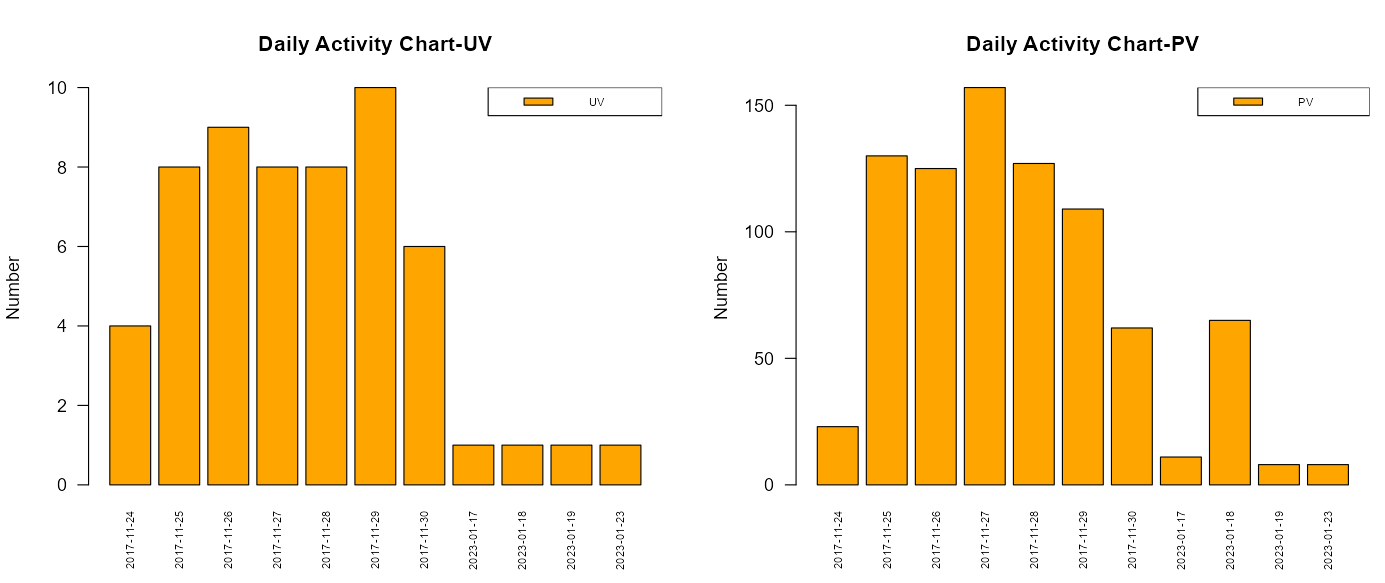
\includegraphics{img/pv_uv.png}

\begin{itemize}
\item
  UV:Unique Visitor, basic indicators for evaluating user activity on
  network platforms
\item
  PV: Page Views
\end{itemize}

\begin{Shaded}
\begin{Highlighting}[]
\NormalTok{user\_activity\_daily }\OtherTok{\textless{}{-}} \ControlFlowTok{function}\NormalTok{(data)\{}
\NormalTok{  activity }\OtherTok{\textless{}{-}}\NormalTok{ data }\SpecialCharTok{\%\textgreater{}\%}
    \FunctionTok{group\_by}\NormalTok{(date) }\SpecialCharTok{\%\textgreater{}\%}
    \FunctionTok{summarize}\NormalTok{(}\AttributeTok{UV =} \FunctionTok{n\_distinct}\NormalTok{(user\_id), }\AttributeTok{PV =} \FunctionTok{n}\NormalTok{())}
  \FunctionTok{return}\NormalTok{ (activity)}
\NormalTok{\}}
\end{Highlighting}
\end{Shaded}

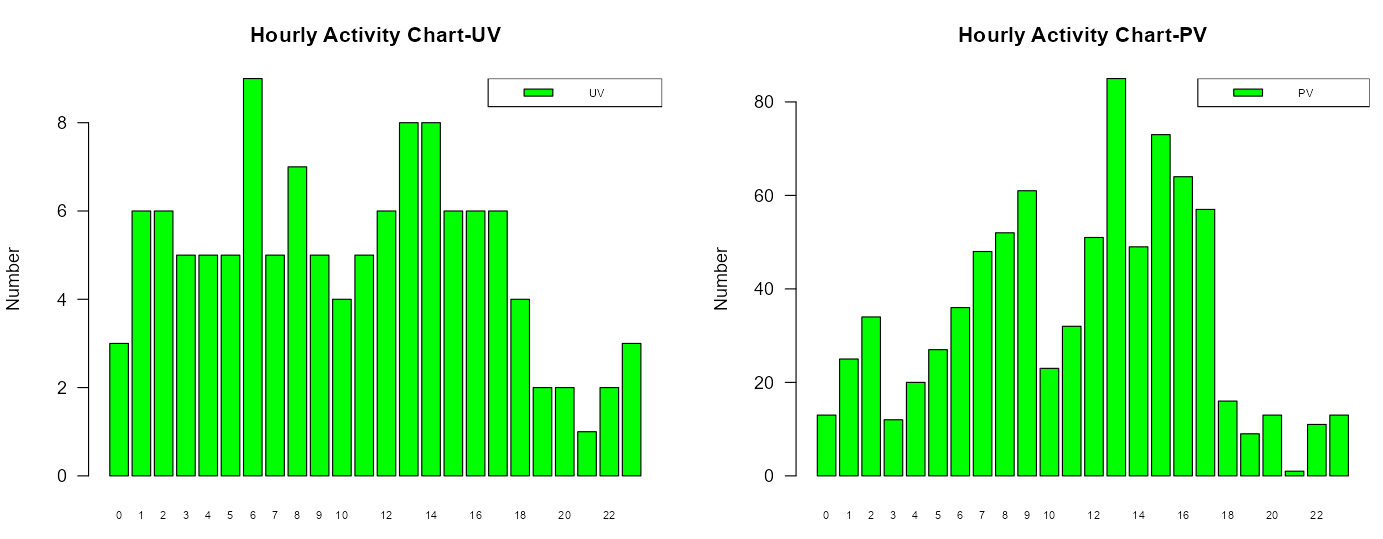
\includegraphics{img/pv_uv_2.png}

\begin{Shaded}
\begin{Highlighting}[]
\NormalTok{user\_activity\_hour }\OtherTok{\textless{}{-}} \ControlFlowTok{function}\NormalTok{(data)\{}
\NormalTok{    hour }\OtherTok{\textless{}{-}}\NormalTok{ data }\SpecialCharTok{\%\textgreater{}\%}
      \FunctionTok{group\_by}\NormalTok{(hour) }\SpecialCharTok{\%\textgreater{}\%}
      \FunctionTok{summarize}\NormalTok{(}\AttributeTok{UV =} \FunctionTok{n\_distinct}\NormalTok{(user\_id), }\AttributeTok{PV =} \FunctionTok{n}\NormalTok{())}
    \FunctionTok{return}\NormalTok{ (hour)}
\NormalTok{  \}}
\end{Highlighting}
\end{Shaded}

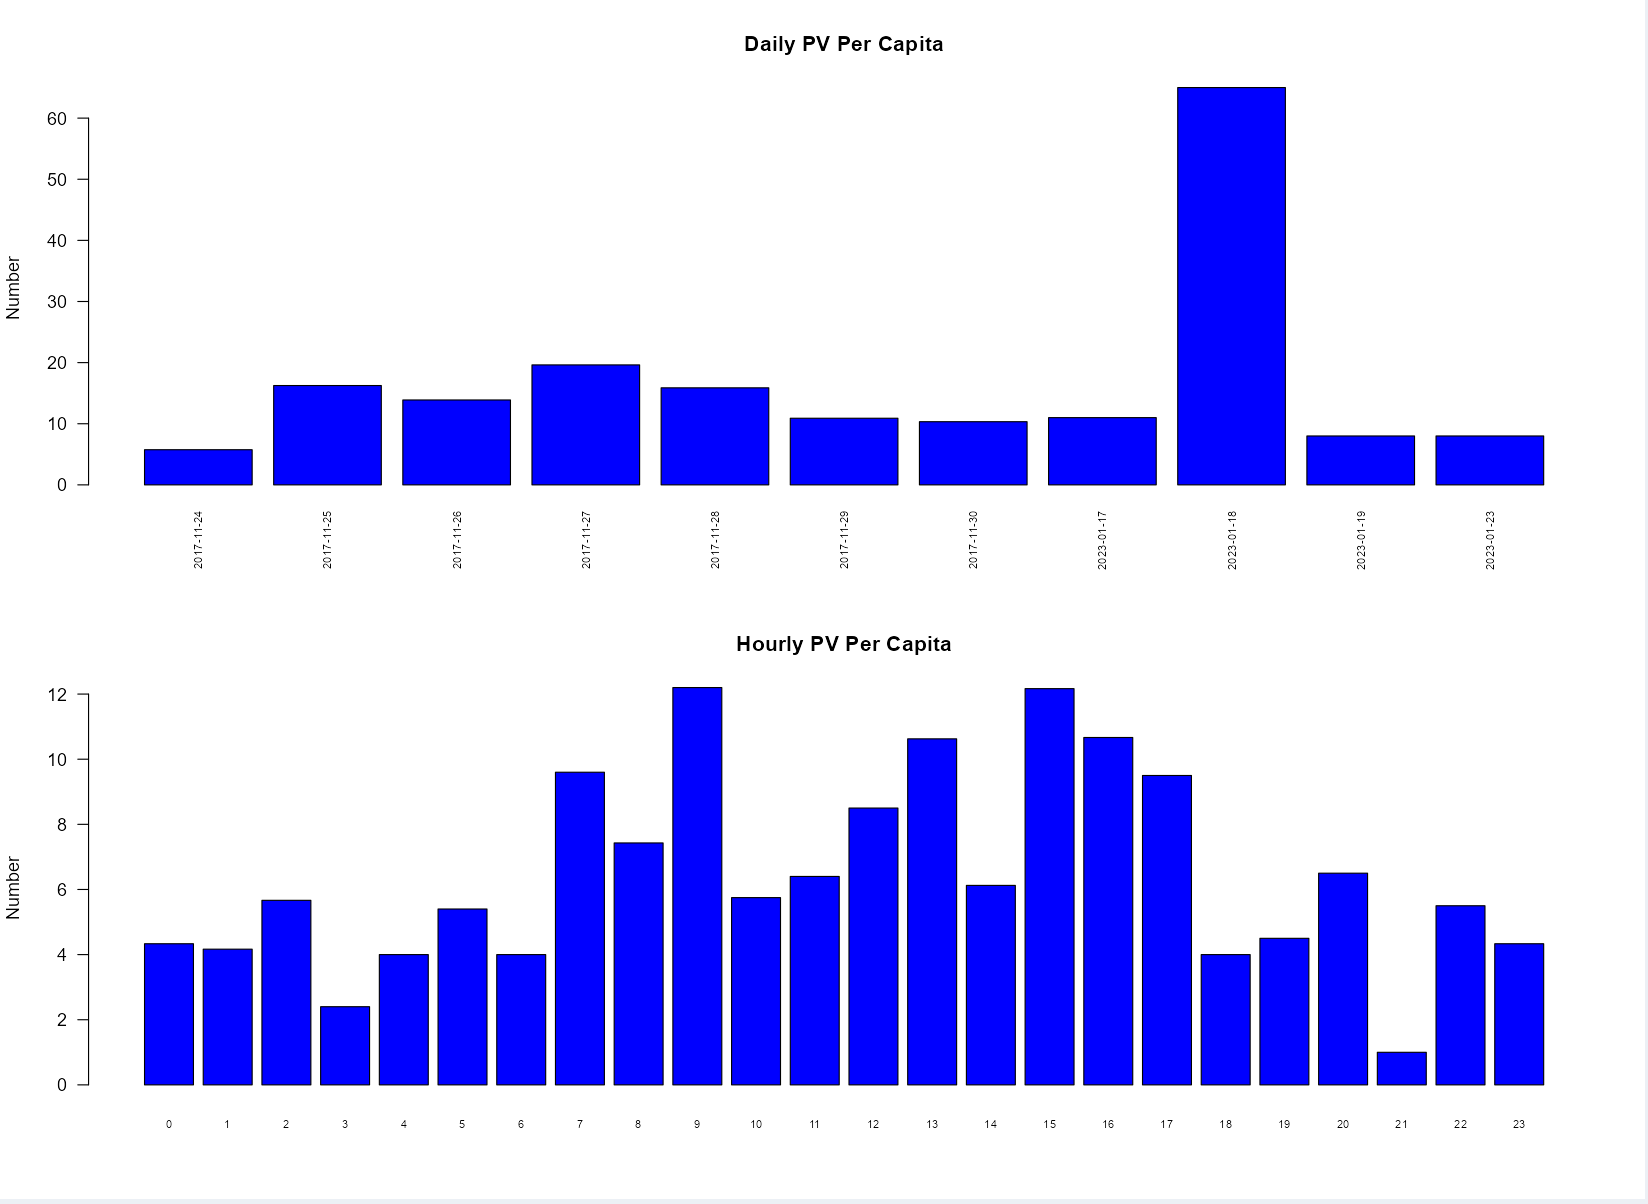
\includegraphics{img/pvuv3.png}

Understand the stickiness of customers to ebuy platform, and count the
daily and hourly per capita PV value.

\begin{Shaded}
\begin{Highlighting}[]
\NormalTok{average\_pv1 }\OtherTok{\textless{}{-}} \ControlFlowTok{function}\NormalTok{(data)\{}
\NormalTok{  average1 }\OtherTok{\textless{}{-}}
\NormalTok{    data }\SpecialCharTok{\%\textgreater{}\%}
    \FunctionTok{group\_by}\NormalTok{(date) }\SpecialCharTok{\%\textgreater{}\%}
    \FunctionTok{summarize}\NormalTok{(}\AttributeTok{UV =} \FunctionTok{n\_distinct}\NormalTok{(user\_id), }\AttributeTok{PV =} \FunctionTok{n}\NormalTok{()) }\SpecialCharTok{\%\textgreater{}\%}
    \FunctionTok{mutate}\NormalTok{(}\AttributeTok{PVmeandaily =}\NormalTok{ PV}\SpecialCharTok{/}\NormalTok{UV)}
  \FunctionTok{return}\NormalTok{(average1)}
\NormalTok{\}}
\NormalTok{average\_pv2 }\OtherTok{\textless{}{-}} \ControlFlowTok{function}\NormalTok{(data)\{}
\NormalTok{  average2 }\OtherTok{\textless{}{-}}
\NormalTok{    data }\SpecialCharTok{\%\textgreater{}\%}
    \FunctionTok{group\_by}\NormalTok{(hour) }\SpecialCharTok{\%\textgreater{}\%}
    \FunctionTok{summarize}\NormalTok{(}\AttributeTok{UV =} \FunctionTok{n\_distinct}\NormalTok{(user\_id), }\AttributeTok{PV =} \FunctionTok{n}\NormalTok{()) }\SpecialCharTok{\%\textgreater{}\%}
    \FunctionTok{mutate}\NormalTok{(}\AttributeTok{PVmeanhourly =}\NormalTok{ PV}\SpecialCharTok{/}\NormalTok{UV)}
  \FunctionTok{return}\NormalTok{(average2)}
\NormalTok{\}}
\end{Highlighting}
\end{Shaded}

\hypertarget{order-data-analysis}{%
\subsection{Order data analysis}\label{order-data-analysis}}

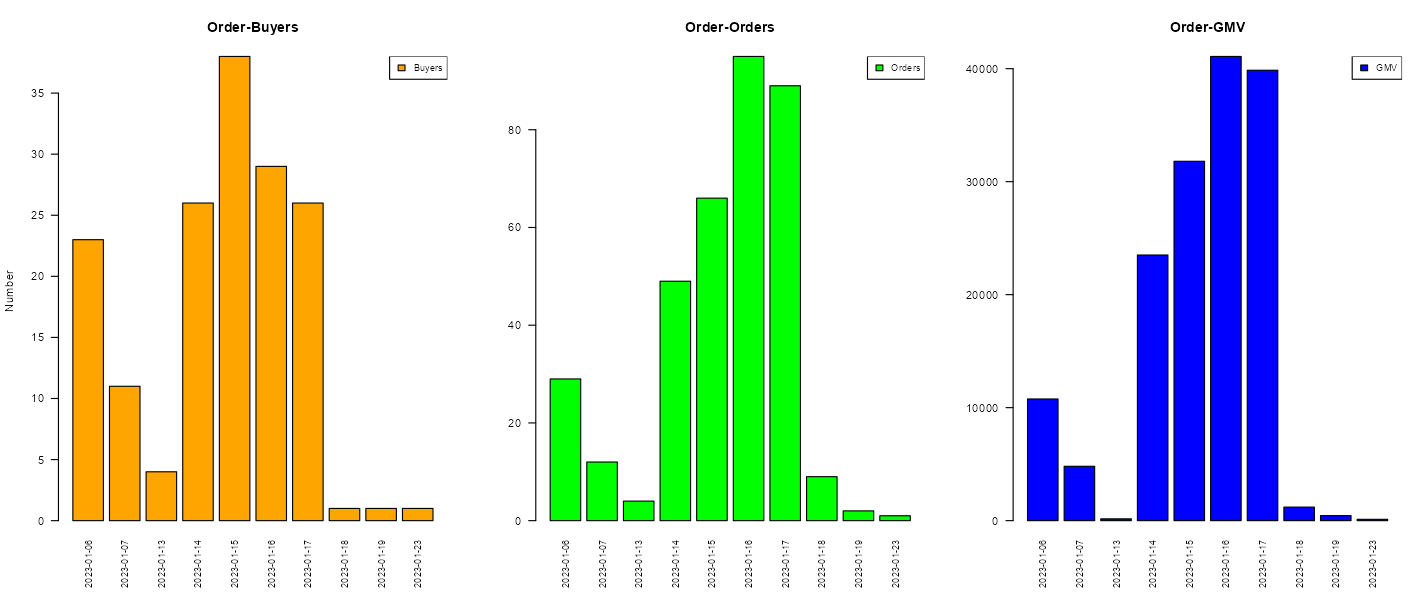
\includegraphics{img/order.png}

\begin{itemize}
\item
  How many orders are generated every day?
\item
  How many GMV(Gross Merchandise Volume)per day?
\end{itemize}

\textbf{The answer is ``User order data graph''}

Why GMV is important ?

\begin{enumerate}
\def\labelenumi{\arabic{enumi}.}
\item
  Performance measurement: GMV provides an overall measure of the scale
  and growth of a platform's business. It helps track the platform's
  sales performance and evaluate its success in attracting buyers and
  sellers.
\item
  Revenue generation: Many online marketplaces generate revenue by
  charging fees or commissions based on a percentage of the GMV. Thus,
  GMV directly impacts the platform's revenue potential.
\item
  Market share comparison: GMV allows comparisons between different
  e-commerce platforms or online marketplaces. It helps investors,
  analysts, and stakeholders assess the market presence and
  competitiveness of a platform relative to its peers.
\item
  Valuation: GMV is sometimes used as a key factor in valuing e-commerce
  businesses, especially in startup or investment scenarios. Higher GMV
  figures can positively influence the valuation of a platform.
\end{enumerate}

\begin{Shaded}
\begin{Highlighting}[]
\NormalTok{user\_order }\OtherTok{\textless{}{-}} \ControlFlowTok{function}\NormalTok{(data)\{}
\NormalTok{  user }\OtherTok{\textless{}{-}}\NormalTok{  data }\SpecialCharTok{\%\textgreater{}\%}
    \FunctionTok{group\_by}\NormalTok{(date) }\SpecialCharTok{\%\textgreater{}\%}
    \FunctionTok{summarise}\NormalTok{(}\AttributeTok{distinct\_users =} \FunctionTok{n\_distinct}\NormalTok{(user\_id),}
              \AttributeTok{total\_products =} \FunctionTok{n}\NormalTok{(),}
              \AttributeTok{total\_price =} \FunctionTok{sum}\NormalTok{(product\_price))}
  \FunctionTok{return}\NormalTok{(user)}
\NormalTok{\}}
\end{Highlighting}
\end{Shaded}

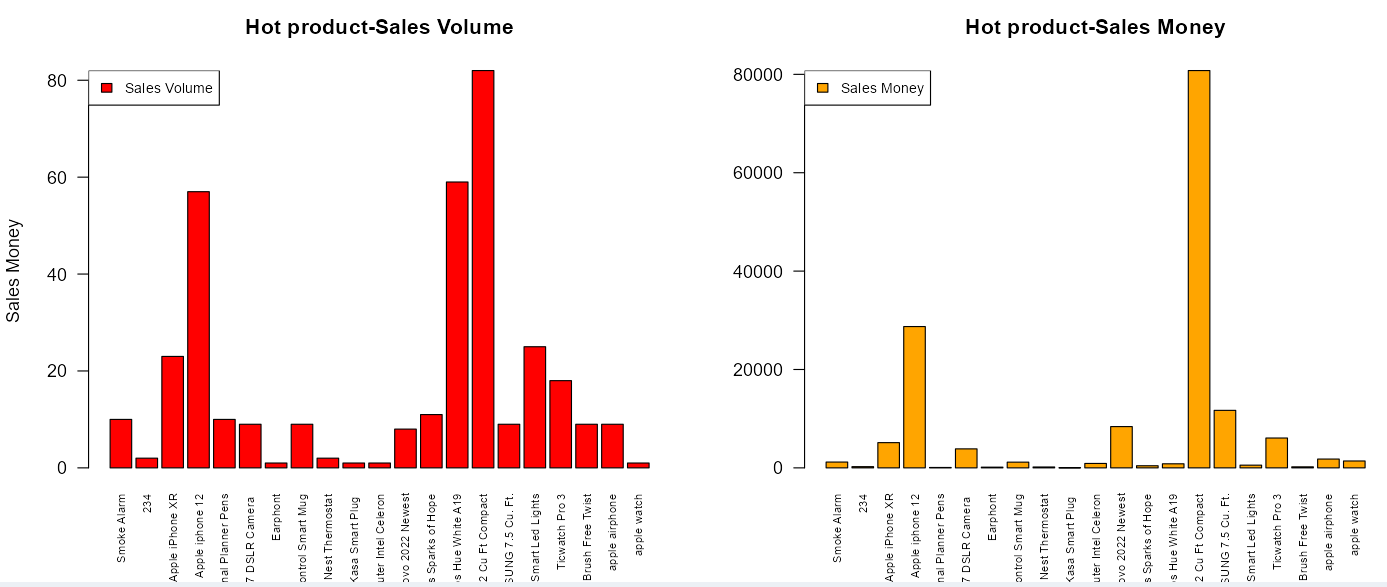
\includegraphics{img/hot.png}

\begin{itemize}
\tightlist
\item
  Want to know which product is the most popular?
\item
  How many sales of hot-selling products per day?
\item
  What is the daily income of hot-selling products?
\end{itemize}

\textbf{The answer is ``Hot product chart''}

\begin{Shaded}
\begin{Highlighting}[]
\NormalTok{hot\_product }\OtherTok{\textless{}{-}} \ControlFlowTok{function}\NormalTok{(data)\{}
\NormalTok{    product }\OtherTok{\textless{}{-}}\NormalTok{ data }\SpecialCharTok{\%\textgreater{}\%}
      \FunctionTok{group\_by}\NormalTok{(product\_name) }\SpecialCharTok{\%\textgreater{}\%}
      \FunctionTok{summarise}\NormalTok{(}\AttributeTok{count\_order =} \FunctionTok{n}\NormalTok{(),}
                \AttributeTok{sum\_product\_price =} \FunctionTok{sum}\NormalTok{(product\_price))}

    \FunctionTok{return}\NormalTok{(product)}
\NormalTok{\}}
\end{Highlighting}
\end{Shaded}

\hypertarget{funnel-model-for-conversion-rate}{%
\subsection{Funnel model for conversion
rate}\label{funnel-model-for-conversion-rate}}

The conversion rate of users in the shopping process is one of the most
important indicators of e-commerce platforms. The higher the conversion
rate, the higher the stickiness of users to the platform.

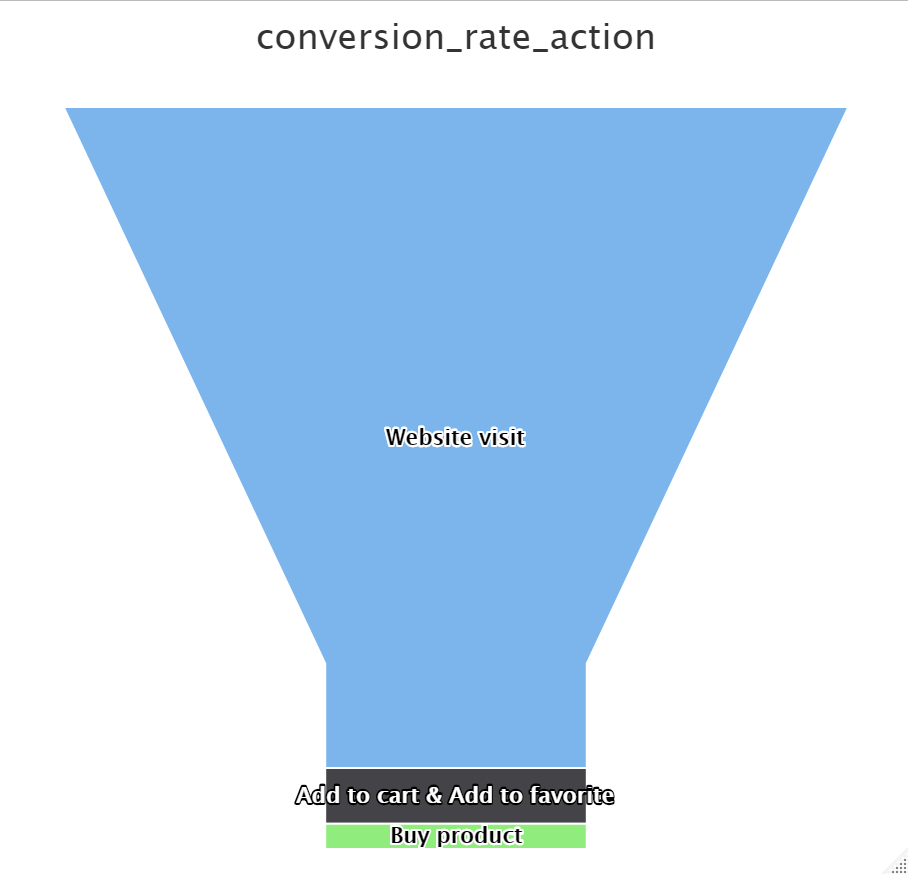
\includegraphics{img/funnel1.png}

\begin{itemize}
\tightlist
\item
  The funnel conversion rate model for user behavior:
\end{itemize}

\begin{Shaded}
\begin{Highlighting}[]
\NormalTok{pv\_sum  }\OtherTok{\textless{}{-}} \FunctionTok{length}\NormalTok{(pv\_data\_object}\SpecialCharTok{@}\NormalTok{behavior\_id)}
\NormalTok{cf\_sum  }\OtherTok{\textless{}{-}} \FunctionTok{length}\NormalTok{(cf\_data\_object}\SpecialCharTok{@}\NormalTok{behavior\_id)}
\NormalTok{buy\_sum  }\OtherTok{\textless{}{-}} \FunctionTok{length}\NormalTok{(buy\_data\_object}\SpecialCharTok{@}\NormalTok{behavior\_id)}
\NormalTok{merge\_sum }\OtherTok{\textless{}{-}} \FunctionTok{nrow}\NormalTok{(merged\_data)}

\NormalTok{sum}
\CommentTok{\# Calculating conversion rates}
\NormalTok{convert\_rate\_action }\OtherTok{\textless{}{-}} \FunctionTok{c}\NormalTok{(}\DecValTok{100}\NormalTok{, cf\_sum[[}\DecValTok{1}\NormalTok{]] }\SpecialCharTok{/}\NormalTok{ pv\_sum[[}\DecValTok{1}\NormalTok{]] }\SpecialCharTok{*} \DecValTok{100}\NormalTok{,}
\NormalTok{                         buy\_sum[[}\DecValTok{1}\NormalTok{]] }\SpecialCharTok{/}\NormalTok{ pv\_sum[[}\DecValTok{1}\NormalTok{]] }\SpecialCharTok{*} \DecValTok{100}\NormalTok{)}
\NormalTok{x\_data }\OtherTok{\textless{}{-}} \FunctionTok{c}\NormalTok{(}\StringTok{"Website visit"}\NormalTok{,}
            \StringTok{"Add to cart \& Add to favorite"}\NormalTok{, }\StringTok{"Buy product"}\NormalTok{)}

\CommentTok{\# Creating data for funnel chart}
\NormalTok{data }\OtherTok{\textless{}{-}} \FunctionTok{data.frame}\NormalTok{(}\AttributeTok{name =}\NormalTok{ x\_data, }\AttributeTok{y =}\NormalTok{ convert\_rate\_action)}

\CommentTok{\# Creating funnel chart}
\NormalTok{hc }\OtherTok{\textless{}{-}} \FunctionTok{highchart}\NormalTok{() }\SpecialCharTok{\%\textgreater{}\%}
  \FunctionTok{hc\_chart}\NormalTok{(}\AttributeTok{type =} \StringTok{"funnel"}\NormalTok{) }\SpecialCharTok{\%\textgreater{}\%}
  \FunctionTok{hc\_title}\NormalTok{(}\AttributeTok{text =} \StringTok{"conversion\_rate\_action"}\NormalTok{,}
           \AttributeTok{subtitle =} \StringTok{"Browse {-}{-}\textgreater{} Purchase\&Favorite {-}{-}\textgreater{} Purchase"}\NormalTok{) }\SpecialCharTok{\%\textgreater{}\%}
  \FunctionTok{hc\_add\_series}\NormalTok{(}\AttributeTok{data =}\NormalTok{ data,}
                \AttributeTok{type =} \StringTok{"funnel"}\NormalTok{,}
                \AttributeTok{name =} \StringTok{""}\NormalTok{,}
                \AttributeTok{dataLabels =} \FunctionTok{list}\NormalTok{(}\AttributeTok{enabled =} \ConstantTok{TRUE}\NormalTok{, }\AttributeTok{inside =} \ConstantTok{TRUE}\NormalTok{),}
                \AttributeTok{tooltip =} \FunctionTok{list}\NormalTok{(}\AttributeTok{pointFormat =} \StringTok{"\{point.name\}: \{point.y\}\%"}\NormalTok{),}
                \AttributeTok{borderColor =} \StringTok{"\#fff"}\NormalTok{,}
                \AttributeTok{borderWidth =} \DecValTok{1}\NormalTok{)}
\end{Highlighting}
\end{Shaded}

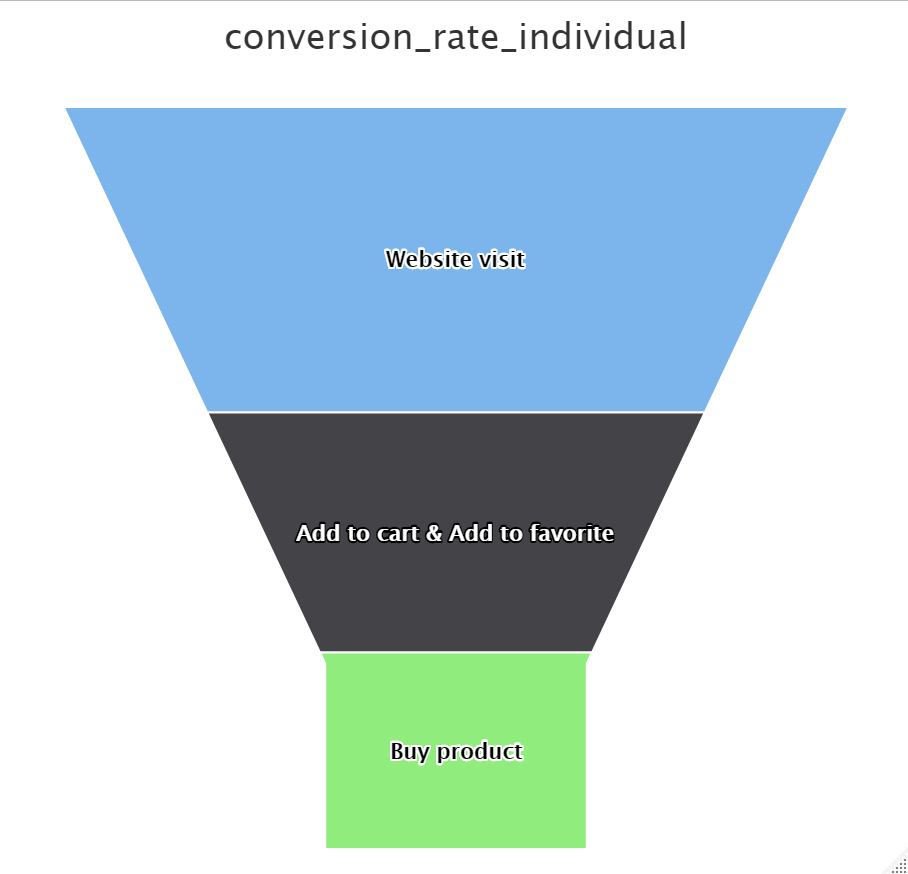
\includegraphics{img/funnel2.png}

\begin{itemize}
\tightlist
\item
  The funnel conversion rate model for individual users:
\end{itemize}

\begin{Shaded}
\begin{Highlighting}[]
\NormalTok{pv\_sum  }\OtherTok{\textless{}{-}} \FunctionTok{length}\NormalTok{(pv\_data\_object}\SpecialCharTok{@}\NormalTok{behavior\_id)}
\NormalTok{cf\_sum  }\OtherTok{\textless{}{-}} \FunctionTok{length}\NormalTok{(cf\_data\_object}\SpecialCharTok{@}\NormalTok{behavior\_id)}
\NormalTok{buy\_sum  }\OtherTok{\textless{}{-}} \FunctionTok{length}\NormalTok{(buy\_data\_object}\SpecialCharTok{@}\NormalTok{behavior\_id)}
\NormalTok{merge\_sum }\OtherTok{\textless{}{-}} \FunctionTok{nrow}\NormalTok{(merged\_data)}

\NormalTok{sum}
\CommentTok{\# Calculating conversion rates}
\NormalTok{convert\_rate\_action }\OtherTok{\textless{}{-}} \FunctionTok{c}\NormalTok{(}\DecValTok{100}\NormalTok{,}
\NormalTok{                         cf\_sum[[}\DecValTok{1}\NormalTok{]] }\SpecialCharTok{/}\NormalTok{ pv\_sum[[}\DecValTok{1}\NormalTok{]] }\SpecialCharTok{*} \DecValTok{100}\NormalTok{,}
\NormalTok{                         buy\_sum[[}\DecValTok{1}\NormalTok{]] }\SpecialCharTok{/}\NormalTok{ pv\_sum[[}\DecValTok{1}\NormalTok{]] }\SpecialCharTok{*} \DecValTok{100}\NormalTok{)}
\NormalTok{x\_data }\OtherTok{\textless{}{-}} \FunctionTok{c}\NormalTok{(}\StringTok{"Website visit"}\NormalTok{, }\StringTok{"Add to cart \& Add to favorite"}\NormalTok{, }\StringTok{"Buy product"}\NormalTok{)}

\CommentTok{\# Creating data for funnel chart}
\NormalTok{data }\OtherTok{\textless{}{-}} \FunctionTok{data.frame}\NormalTok{(}\AttributeTok{name =}\NormalTok{ x\_data, }\AttributeTok{y =}\NormalTok{ convert\_rate\_action)}

\CommentTok{\# Creating funnel chart}
\NormalTok{hc }\OtherTok{\textless{}{-}} \FunctionTok{highchart}\NormalTok{() }\SpecialCharTok{\%\textgreater{}\%}
  \FunctionTok{hc\_chart}\NormalTok{(}\AttributeTok{type =} \StringTok{"funnel"}\NormalTok{) }\SpecialCharTok{\%\textgreater{}\%}
  \FunctionTok{hc\_title}\NormalTok{(}\AttributeTok{text =} \StringTok{"conversion\_rate\_action"}\NormalTok{,}
           \AttributeTok{subtitle =} \StringTok{"Browse {-}{-}\textgreater{} Purchase\&Favorite {-}{-}\textgreater{} Purchase"}\NormalTok{) }\SpecialCharTok{\%\textgreater{}\%}
  \FunctionTok{hc\_add\_series}\NormalTok{(}\AttributeTok{data =}\NormalTok{ data,}
                \AttributeTok{type =} \StringTok{"funnel"}\NormalTok{,}
                \AttributeTok{name =} \StringTok{""}\NormalTok{,}
                \AttributeTok{dataLabels =} \FunctionTok{list}\NormalTok{(}\AttributeTok{enabled =} \ConstantTok{TRUE}\NormalTok{, }\AttributeTok{inside =} \ConstantTok{TRUE}\NormalTok{),}
                \AttributeTok{tooltip =} \FunctionTok{list}\NormalTok{(}\AttributeTok{pointFormat =} \StringTok{"\{point.name\}: \{point.y\}\%"}\NormalTok{),}
                \AttributeTok{borderColor =} \StringTok{"\#fff"}\NormalTok{,}\AttributeTok{borderWidth =} \DecValTok{1}\NormalTok{)}
\end{Highlighting}
\end{Shaded}

\hypertarget{consumer-segmentation-using-k-means-and-rfm}{%
\subsection{Consumer segmentation using K-Means and
RFM}\label{consumer-segmentation-using-k-means-and-rfm}}

RFM: marketing technique used to quantitatively rank and group customers
based on the recency, frequency and monetary total of their recent
transactions to identify the best customers and perform targeted
marketing campaigns. RFM analysis is based on the marketing adage that
``80\% of your business comes from 20\% of your customers.''

\begin{itemize}
\tightlist
\item
  Recency. How recent was the customer's last purchase?
\item
  Frequency. How often did this customer make a purchase in a given
  period?
\item
  Monetary. How much money did the customer spend in a given period?
\end{itemize}

Then, using K-Means to cluster our consumer.

\begin{itemize}
\tightlist
\item
  firstly, z-score standardization helps to adjust all data elements to
  a common scale to improve the performance of clustering algorithms.
\item
  using K-Means, I directly set 3 clusters.
\end{itemize}

\begin{Shaded}
\begin{Highlighting}[]
\NormalTok{scaled\_data }\OtherTok{\textless{}{-}}\NormalTok{ k\_mean\_data }\SpecialCharTok{\%\textgreater{}\%}
  \FunctionTok{select}\NormalTok{(}\SpecialCharTok{{-}}\NormalTok{user\_id) }\SpecialCharTok{\%\textgreater{}\%}
  \FunctionTok{scale}\NormalTok{()}

\CommentTok{\# Perform k{-}means clustering}
\NormalTok{k }\OtherTok{\textless{}{-}} \DecValTok{3}  \CommentTok{\# Number of clusters}
\NormalTok{kmeans\_result }\OtherTok{\textless{}{-}} \FunctionTok{kmeans}\NormalTok{(scaled\_data, }\AttributeTok{centers =}\NormalTok{ k, }\AttributeTok{nstart =} \DecValTok{10}\NormalTok{)}

\CommentTok{\# Get cluster assignments and cluster centers}
\NormalTok{clusters }\OtherTok{\textless{}{-}}\NormalTok{ kmeans\_result}\SpecialCharTok{$}\NormalTok{cluster}
\NormalTok{centroids }\OtherTok{\textless{}{-}}\NormalTok{ kmeans\_result}\SpecialCharTok{$}\NormalTok{centers}

\CommentTok{\# Add cluster assignments to the dataframe}
\NormalTok{k\_mean\_data}\SpecialCharTok{$}\NormalTok{group }\OtherTok{\textless{}{-}}\NormalTok{ clusters}
\end{Highlighting}
\end{Shaded}

Then, the classification results are displayed. Use the radar map to
illustrate the classification method.

\begin{itemize}
\item
  group1: the time since the last consumption is the shortest, although
  the frequency and monetary are low, but the consumption has been
  relatively active, they can be motivated by some promotional tools.
\item
  group3: customers are the frequency and monetary are the largest. They
  are high-value customers and need to be maintained.
\item
  group2: worst consumption behaviors. They are likely to be churned
  customers and
\item
  need to be activated
\end{itemize}

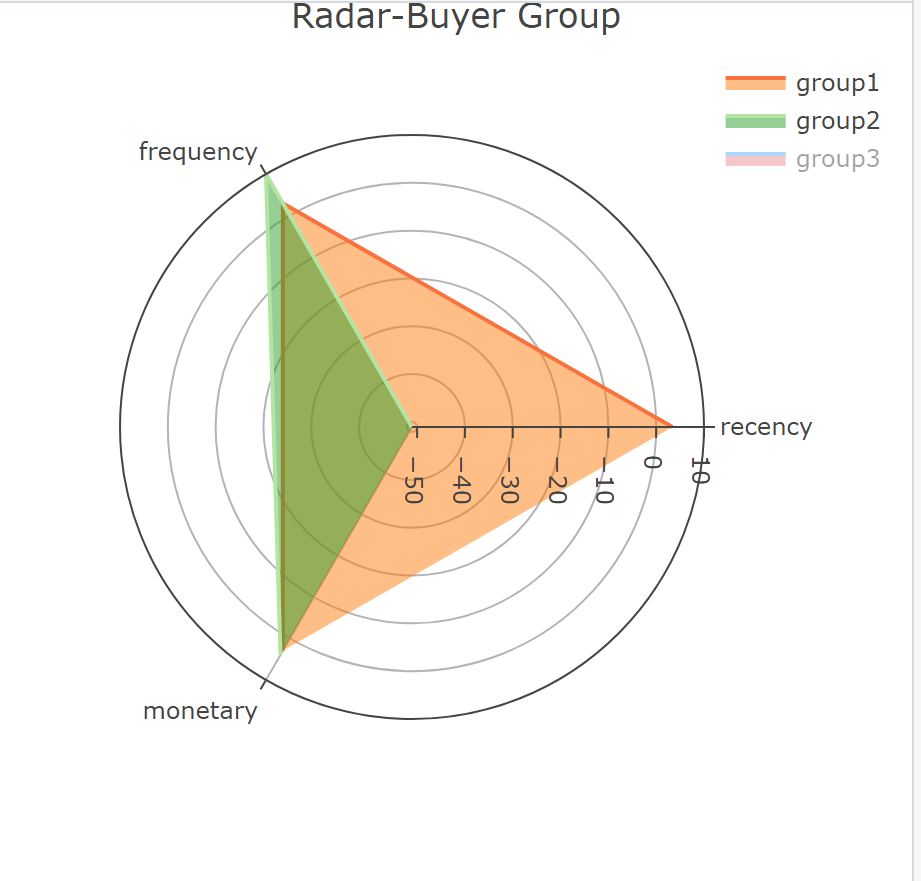
\includegraphics{img/radar1.png}

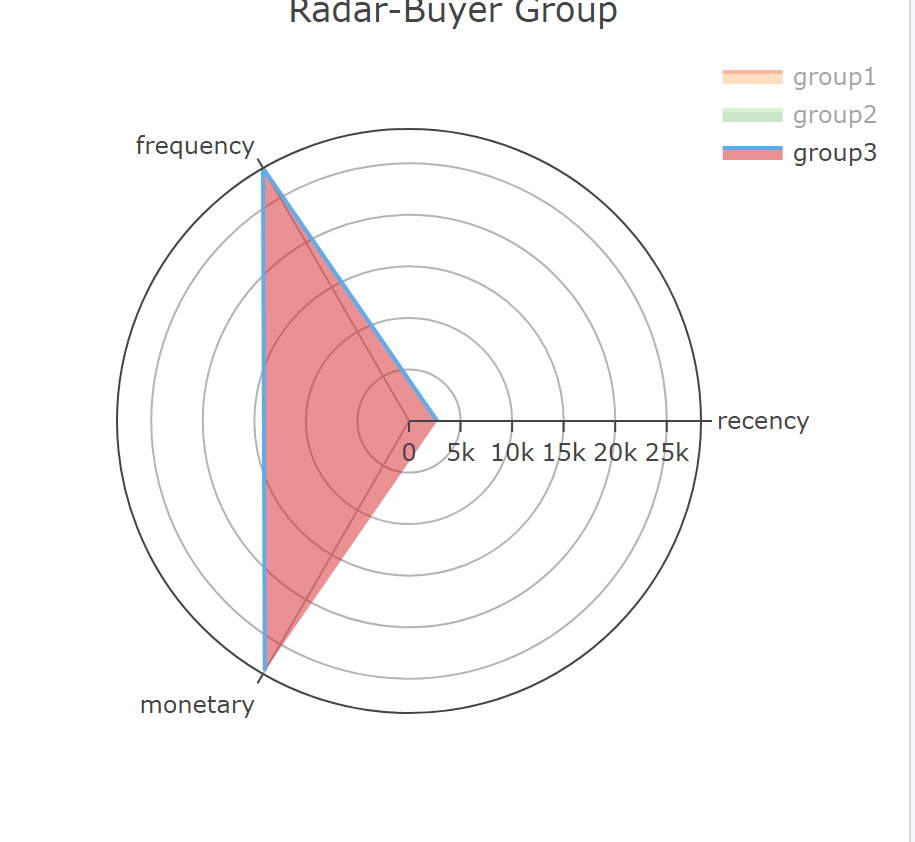
\includegraphics{img/radar2.png}

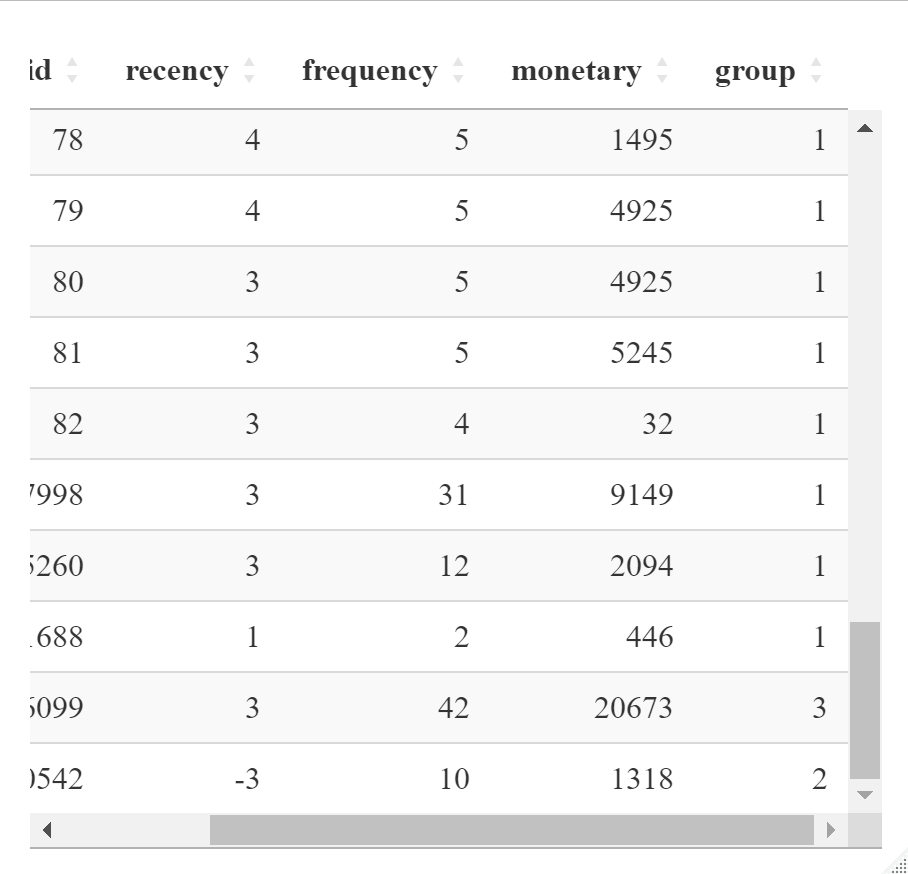
\includegraphics{img/table1.png}

\begin{Shaded}
\begin{Highlighting}[]
\NormalTok{centroids\_restored }\OtherTok{\textless{}{-}}\NormalTok{ centroids }\SpecialCharTok{*} \FunctionTok{attr}\NormalTok{(scaled\_data, }\StringTok{"scaled:scale"}\NormalTok{)}
\SpecialCharTok{+} \FunctionTok{attr}\NormalTok{(scaled\_data, }\StringTok{"scaled:center"}\NormalTok{)}

\CommentTok{\# Plot the radar chart}
\NormalTok{group1 }\OtherTok{\textless{}{-}} \FunctionTok{as.list}\NormalTok{(centroids\_restored[}\DecValTok{1}\NormalTok{, ])}
\NormalTok{group2 }\OtherTok{\textless{}{-}} \FunctionTok{as.list}\NormalTok{(centroids\_restored[}\DecValTok{2}\NormalTok{, ])}
\NormalTok{group3 }\OtherTok{\textless{}{-}} \FunctionTok{as.list}\NormalTok{(centroids\_restored[}\DecValTok{3}\NormalTok{, ])}

\NormalTok{radar }\OtherTok{\textless{}{-}} \FunctionTok{plot\_ly}\NormalTok{(}\AttributeTok{type =} \StringTok{\textquotesingle{}scatterpolar\textquotesingle{}}\NormalTok{, }\AttributeTok{mode =} \StringTok{\textquotesingle{}lines\textquotesingle{}}\NormalTok{)}

\NormalTok{radar }\OtherTok{\textless{}{-}} \FunctionTok{add\_trace}\NormalTok{(}
\NormalTok{  radar,}
  \AttributeTok{r =} \FunctionTok{c}\NormalTok{(group1}\SpecialCharTok{$}\NormalTok{recency, group1}\SpecialCharTok{$}\NormalTok{frequency, group1}\SpecialCharTok{$}\NormalTok{monetary),}
  \AttributeTok{theta =} \FunctionTok{c}\NormalTok{(}\StringTok{\textquotesingle{}recency\textquotesingle{}}\NormalTok{, }\StringTok{\textquotesingle{}frequency\textquotesingle{}}\NormalTok{, }\StringTok{\textquotesingle{}monetary\textquotesingle{}}\NormalTok{),}
  \AttributeTok{fill =} \StringTok{\textquotesingle{}toself\textquotesingle{}}\NormalTok{,}
  \AttributeTok{name =} \StringTok{\textquotesingle{}group1\textquotesingle{}}\NormalTok{,}
  \AttributeTok{line =} \FunctionTok{list}\NormalTok{(}\AttributeTok{color =} \StringTok{\textquotesingle{}\#f9713c\textquotesingle{}}\NormalTok{)}
\NormalTok{)}

\NormalTok{radar }\OtherTok{\textless{}{-}} \FunctionTok{add\_trace}\NormalTok{(}
\NormalTok{  radar,}
  \AttributeTok{r =} \FunctionTok{c}\NormalTok{(group2}\SpecialCharTok{$}\NormalTok{recency, group2}\SpecialCharTok{$}\NormalTok{frequency, group2}\SpecialCharTok{$}\NormalTok{monetary),}
  \AttributeTok{theta =} \FunctionTok{c}\NormalTok{(}\StringTok{\textquotesingle{}recency\textquotesingle{}}\NormalTok{, }\StringTok{\textquotesingle{}frequency\textquotesingle{}}\NormalTok{, }\StringTok{\textquotesingle{}monetary\textquotesingle{}}\NormalTok{),}
  \AttributeTok{fill =} \StringTok{\textquotesingle{}toself\textquotesingle{}}\NormalTok{,}
  \AttributeTok{name =} \StringTok{\textquotesingle{}group2\textquotesingle{}}\NormalTok{,}
  \AttributeTok{line =} \FunctionTok{list}\NormalTok{(}\AttributeTok{color =} \StringTok{\textquotesingle{}\#b3e4a1\textquotesingle{}}\NormalTok{)}
\NormalTok{)}

\NormalTok{radar }\OtherTok{\textless{}{-}} \FunctionTok{add\_trace}\NormalTok{(}
\NormalTok{  radar,}
  \AttributeTok{r =} \FunctionTok{c}\NormalTok{(group3}\SpecialCharTok{$}\NormalTok{recency, group3}\SpecialCharTok{$}\NormalTok{frequency, group3}\SpecialCharTok{$}\NormalTok{monetary),}
  \AttributeTok{theta =} \FunctionTok{c}\NormalTok{(}\StringTok{\textquotesingle{}recency\textquotesingle{}}\NormalTok{, }\StringTok{\textquotesingle{}frequency\textquotesingle{}}\NormalTok{, }\StringTok{\textquotesingle{}monetary\textquotesingle{}}\NormalTok{),}
  \AttributeTok{fill =} \StringTok{\textquotesingle{}toself\textquotesingle{}}\NormalTok{,}
  \AttributeTok{name =} \StringTok{\textquotesingle{}group3\textquotesingle{}}\NormalTok{,}
  \AttributeTok{line =} \FunctionTok{list}\NormalTok{(}\AttributeTok{color =} \StringTok{\textquotesingle{}\#5CACEE\textquotesingle{}}\NormalTok{)}
\NormalTok{)}

\NormalTok{radar }\OtherTok{\textless{}{-}} \FunctionTok{layout}\NormalTok{(}
\NormalTok{  radar,}
  \AttributeTok{title =} \StringTok{\textquotesingle{}Radar{-}Buyer Group\textquotesingle{}}\NormalTok{,}
  \AttributeTok{showlegend =} \ConstantTok{TRUE}
\NormalTok{)}
\end{Highlighting}
\end{Shaded}

\hypertarget{future-order-forcast}{%
\subsection{Future Order Forcast}\label{future-order-forcast}}

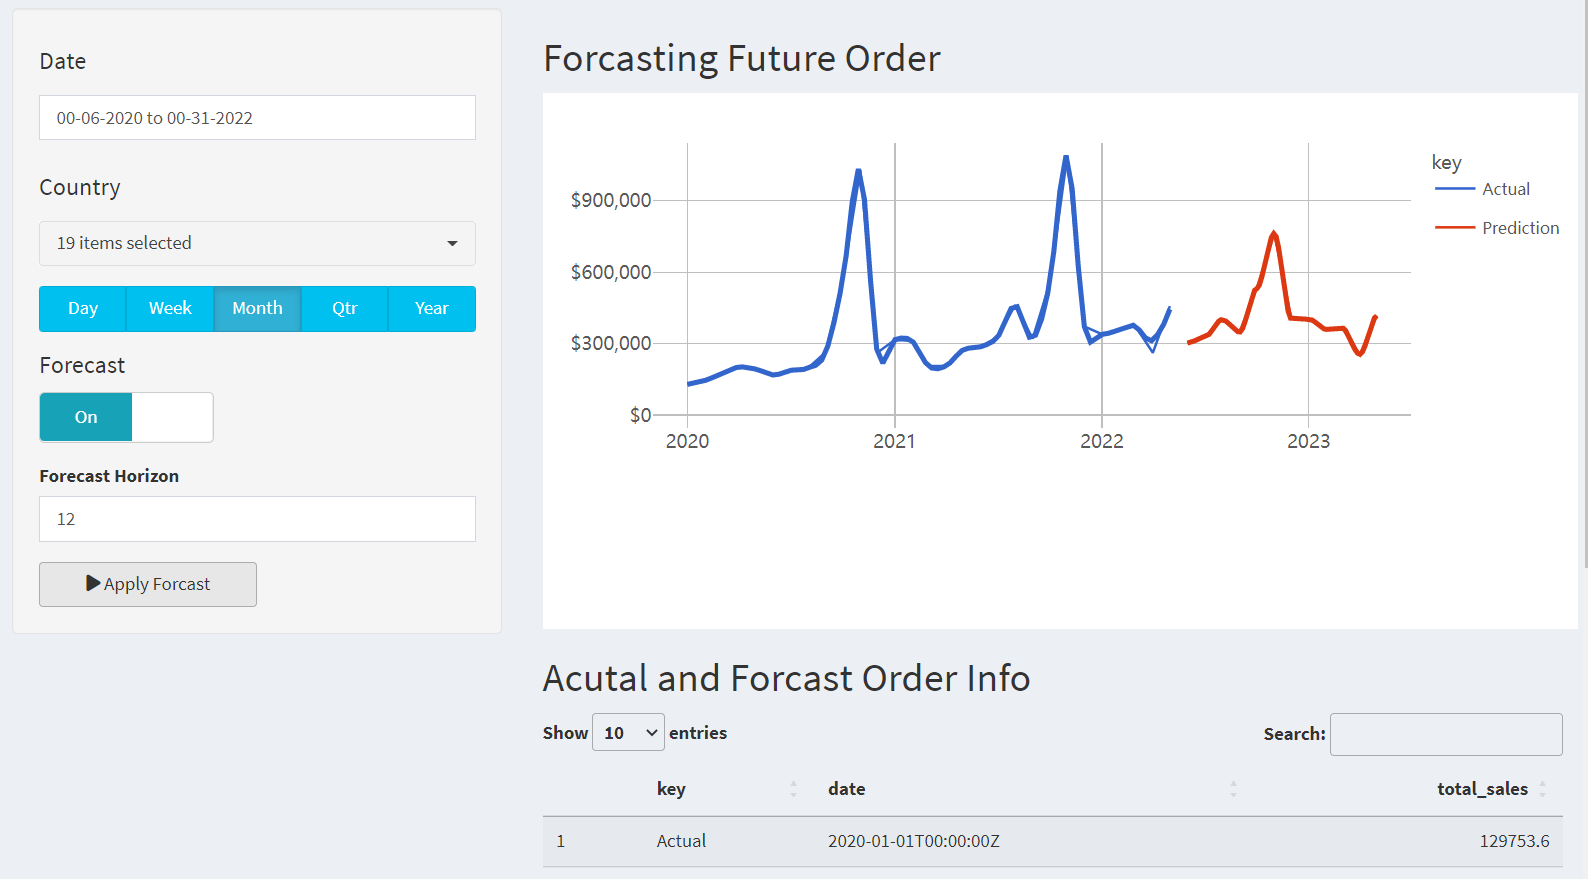
\includegraphics{img/page1.png}

Future order forecasting page was incorporated the shiny dashboard
library for the sidebar layout. Graphs and figures were created using
the ggplot2 library and data table.

\hypertarget{data-preprocessing}{%
\subsubsection{Data Preprocessing}\label{data-preprocessing}}

\begin{Shaded}
\begin{Highlighting}[]
\CommentTok{\# Load data}
\NormalTok{sales\_data\_raw }\OtherTok{\textless{}{-}} \FunctionTok{read\_csv}\NormalTok{(}\StringTok{\textquotesingle{}data/orders02.csv\textquotesingle{}}\NormalTok{)}

\CommentTok{\# Select relevant data}
\NormalTok{processed\_data\_tbl }\OtherTok{\textless{}{-}}\NormalTok{ sales\_data\_raw }\SpecialCharTok{\%\textgreater{}\%}
  \FunctionTok{select}\NormalTok{(ORDERDATE, ORDERNUMBER, ORDERLINENUMBER,}
\NormalTok{         COUNTRY, SALES, PRODUCTLINE,}
\NormalTok{         DEALSIZE, STATUS, CUSTOMERNAME)}

\CommentTok{\# Pre{-}processing}
\NormalTok{processed\_data\_tbl }\OtherTok{\textless{}{-}}\NormalTok{ processed\_data\_tbl }\SpecialCharTok{\%\textgreater{}\%}
  \FunctionTok{mutate}\NormalTok{(}\AttributeTok{ORDERDATE =} \FunctionTok{mdy\_hm}\NormalTok{(ORDERDATE),}
         \AttributeTok{ORDERDATE =} \FunctionTok{as\_datetime}\NormalTok{(ORDERDATE))}

\CommentTok{\# Manual edits}
\NormalTok{processed\_data\_tbl}\SpecialCharTok{$}\NormalTok{COUNTRY[processed\_data\_tbl}\SpecialCharTok{$}\NormalTok{COUNTRY}\SpecialCharTok{==}\StringTok{"UK"}\NormalTok{] }\OtherTok{\textless{}{-}} \StringTok{"United Kingdom"}
\NormalTok{processed\_data\_tbl}\SpecialCharTok{$}\NormalTok{COUNTRY[processed\_data\_tbl}\SpecialCharTok{$}\NormalTok{COUNTRY}\SpecialCharTok{==}\StringTok{"USA"}\NormalTok{] }\OtherTok{\textless{}{-}} \StringTok{"United States"}
\end{Highlighting}
\end{Shaded}

\hypertarget{modeling}{%
\subsubsection{Modeling}\label{modeling}}

To forcast the future order, linear regression can be utilized to
forecast the year order, while a gradient boosting machine (GBM) can be
employed to predict the quarter,month, week, and day order. Gradient
boosting machines are powerful machine learning algorithms that combine
multiple weak prediction models to create a strong ensemble model. In
the case of forecasting the month, week, and day order, a GBM can be
trained using historical data on past order patterns to create a
predictive model that can anticipate the specific month, week, and day
when a customer is likely to place an order.

\begin{Shaded}
\begin{Highlighting}[]
\NormalTok{generate\_forecast }\OtherTok{\textless{}{-}}
\ControlFlowTok{function}\NormalTok{(data, }\AttributeTok{n\_future =} \DecValTok{12}\NormalTok{, }\AttributeTok{seed =} \ConstantTok{NULL}\NormalTok{) \{}

\NormalTok{  train\_tbl }\OtherTok{\textless{}{-}}\NormalTok{ data }\SpecialCharTok{\%\textgreater{}\%}
    \FunctionTok{tk\_augment\_timeseries\_signature}\NormalTok{()}

\NormalTok{  future\_data\_tbl }\OtherTok{\textless{}{-}}\NormalTok{ data }\SpecialCharTok{\%\textgreater{}\%}
    \FunctionTok{tk\_index}\NormalTok{() }\SpecialCharTok{\%\textgreater{}\%}
    \FunctionTok{tk\_make\_future\_timeseries}\NormalTok{(}\AttributeTok{n\_future =}\NormalTok{ n\_future,}
                              \AttributeTok{inspect\_weekdays =} \ConstantTok{TRUE}\NormalTok{,}
                              \AttributeTok{inspect\_months =} \ConstantTok{TRUE}\NormalTok{) }\SpecialCharTok{\%\textgreater{}\%}
    \FunctionTok{tk\_get\_timeseries\_signature}\NormalTok{()}

  \CommentTok{\# Isolate and pull scale}
\NormalTok{  time\_scale }\OtherTok{\textless{}{-}}\NormalTok{  data }\SpecialCharTok{\%\textgreater{}\%}
    \FunctionTok{tk\_index}\NormalTok{() }\SpecialCharTok{\%\textgreater{}\%}
    \FunctionTok{tk\_get\_timeseries\_summary}\NormalTok{() }\SpecialCharTok{\%\textgreater{}\%}
    \FunctionTok{pull}\NormalTok{(scale)}

  \CommentTok{\# Linear Regression for "year", XGBoost for other time units}
  \ControlFlowTok{if}\NormalTok{ (time\_scale }\SpecialCharTok{==} \StringTok{"year"}\NormalTok{) \{}

\NormalTok{    model }\OtherTok{\textless{}{-}} \FunctionTok{linear\_reg}\NormalTok{(}\AttributeTok{mode =} \StringTok{"regression"}\NormalTok{) }\SpecialCharTok{\%\textgreater{}\%}
      \FunctionTok{set\_engine}\NormalTok{(}\AttributeTok{engine =} \StringTok{"lm"}\NormalTok{) }\SpecialCharTok{\%\textgreater{}\%}
      \FunctionTok{fit.model\_spec}\NormalTok{(total\_sales }\SpecialCharTok{\textasciitilde{}}\NormalTok{ .,}
                     \AttributeTok{data =}\NormalTok{ train\_tbl }\SpecialCharTok{\%\textgreater{}\%} \FunctionTok{select}\NormalTok{(total\_sales, index.num))}

\NormalTok{  \} }\ControlFlowTok{else}\NormalTok{ \{}
\NormalTok{    seed }\OtherTok{\textless{}{-}}\NormalTok{ seed}
    \FunctionTok{set.seed}\NormalTok{(seed)}
\NormalTok{    model }\OtherTok{\textless{}{-}} \FunctionTok{boost\_tree}\NormalTok{(}
      \AttributeTok{mode =} \StringTok{"regression"}\NormalTok{,}
      \AttributeTok{mtry =} \DecValTok{20}\NormalTok{,}
      \AttributeTok{trees =} \DecValTok{500}\NormalTok{,}
      \AttributeTok{min\_n =} \DecValTok{3}\NormalTok{,}
      \AttributeTok{tree\_depth =} \DecValTok{8}\NormalTok{,}
      \AttributeTok{learn\_rate =} \FloatTok{0.01}\NormalTok{,}
      \AttributeTok{loss\_reduction =} \FloatTok{0.01}\NormalTok{) }\SpecialCharTok{\%\textgreater{}\%}
      \FunctionTok{set\_engine}\NormalTok{(}\AttributeTok{engine =} \StringTok{"xgboost"}\NormalTok{) }\SpecialCharTok{\%\textgreater{}\%}
      \FunctionTok{fit.model\_spec}\NormalTok{(total\_sales }\SpecialCharTok{\textasciitilde{}}\NormalTok{ .,}
                     \AttributeTok{data =}\NormalTok{ train\_tbl }\SpecialCharTok{\%\textgreater{}\%}
                       \FunctionTok{select}\NormalTok{(}\SpecialCharTok{{-}}\NormalTok{date, }\SpecialCharTok{{-}}\NormalTok{label\_text, }\SpecialCharTok{{-}}\NormalTok{diff))}
\NormalTok{  \}}
\end{Highlighting}
\end{Shaded}

\hypertarget{visualization}{%
\subsection{Visualization}\label{visualization}}

\hypertarget{filter-area}{%
\subsubsection{Filter area}\label{filter-area}}

\begin{figure}

{\centering 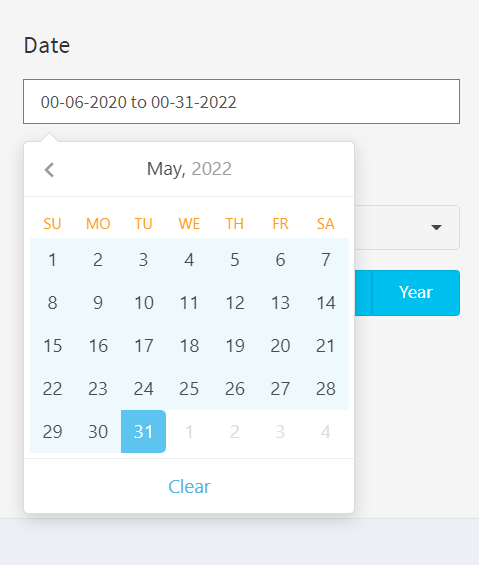
\includegraphics{img/page2.png}

}

\caption{airDatepickerInput}

\end{figure}

\begin{figure}

{\centering 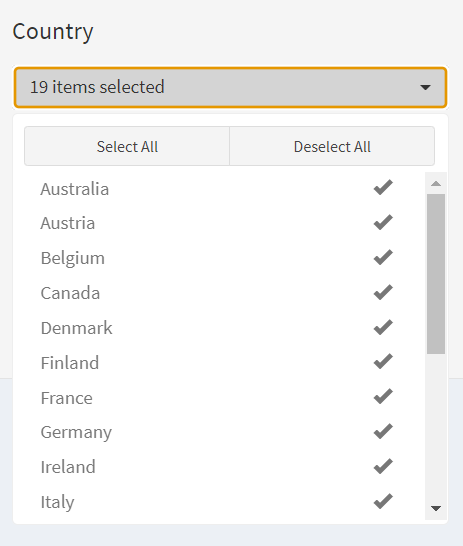
\includegraphics{img/page3.png}

}

\caption{pickerInput}

\end{figure}

\begin{figure}

{\centering 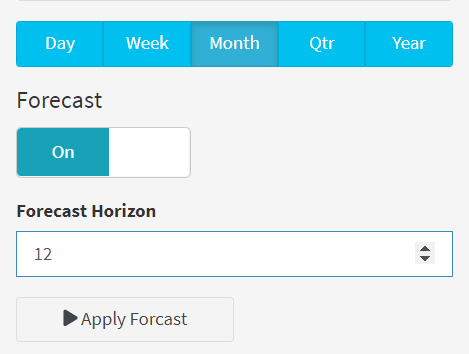
\includegraphics{img/page4.png}

}

\caption{radioGroupButtons}

\end{figure}

The resulting dashboard application allowed users to filter purchase
data, country, choose forcasting time-units(Day, week, month, quarter,
and year) and horizons. For helping businesses identify patterns and
trends in customer order. Code example is as follows:

\begin{Shaded}
\begin{Highlighting}[]
\FunctionTok{library}\NormalTok{(shinyWidgets)}
\FunctionTok{switchInput}\NormalTok{(}\AttributeTok{inputId =} \StringTok{"forecast\_mode"}\NormalTok{,}
            \AttributeTok{handleWidth =} \DecValTok{100}\NormalTok{,}
            \AttributeTok{labelWidth =} \DecValTok{100}\NormalTok{,}
            \AttributeTok{inline =} \ConstantTok{TRUE}\NormalTok{,}
            \AttributeTok{value =} \ConstantTok{FALSE}\NormalTok{,}
            \AttributeTok{onStatus =} \StringTok{"info"}\NormalTok{,}
            \AttributeTok{onLabel =} \StringTok{"On"}\NormalTok{,}
            \AttributeTok{offLabel =} \StringTok{"Off"}\NormalTok{,}
            \AttributeTok{width =} \StringTok{"200px"}\NormalTok{),}

\FunctionTok{conditionalPanel}\NormalTok{(}\AttributeTok{condition =} \StringTok{"input.forecast\_mode == 1"}\NormalTok{,}
                 \FunctionTok{numericInput}\NormalTok{(}\AttributeTok{inputId =} \StringTok{"n\_future"}\NormalTok{,}
                              \AttributeTok{label =} \StringTok{"Forecast Horizon"}\NormalTok{,}
                              \AttributeTok{value =} \DecValTok{12}\NormalTok{,}
                              \AttributeTok{min =} \DecValTok{1}  \CommentTok{\# At least 1 period in the future}
\NormalTok{                 )),}
\CommentTok{\# APPLY BUTTONS {-}{-}{-}{-}{-}}
\FunctionTok{actionButton}\NormalTok{(}\AttributeTok{inputId =} \StringTok{"apply"}\NormalTok{,}
             \AttributeTok{label   =} \StringTok{"Apply Forcast"}\NormalTok{,}
             \AttributeTok{icon    =} \FunctionTok{icon}\NormalTok{(}\StringTok{"play"}\NormalTok{),}
             \AttributeTok{width   =} \StringTok{\textquotesingle{}50\%\textquotesingle{}}\NormalTok{)}
\end{Highlighting}
\end{Shaded}

\hypertarget{reactive-events}{%
\subsubsection{Reactive events}\label{reactive-events}}

Here are several reactive events implemented using different methods:

\begin{itemize}
\item
  Button Click Event: Using the observeEvent method, the reactive code
  is triggered when the user clicks the ``Apply'' button. This means
  that after selecting the data filter, the user needs to manually click
  the button to update the data visualization results.
\item
  Time Unit Button Event: Using the observeEvent method, the reactive
  code is triggered when the user clicks the ``Time Unit'' button,
  simulating the effect of clicking the ``Apply'' button. This means
  that after selecting the time unit, there is no need to manually click
  the ``Apply'' button as the data visualization results will
  automatically update.
\item
  Reactive Expression based on Input: Using the reactive method, a
  reactive expression is created based on user input. The reactive
  expression will automatically recompute and update the data
  visualization results when the input value changes.
\item
  Reactive Event for Forecast Switch: Using the eventReactive method, a
  reactive event is created that triggers when the forecast switch
  status changes. This can be used to execute code related to
  forecasting, such as generating forecast results based on the selected
  time unit.
\end{itemize}

These reactive events differ in terms of how they are triggered and when
the data visualization results are updated. Reactive expressions
automatically recalculate when input values change, while the reactive
event for the forecast switch can execute code related to forecasting
when the switch status changes. These different reactive events enable
the data visualization platform to update and present data in real-time
based on user actions and selections. Code example is as follows:

\begin{Shaded}
\begin{Highlighting}[]
\NormalTok{processed\_data\_filtered\_tbl }\OtherTok{\textless{}{-}} \FunctionTok{eventReactive}\NormalTok{(}
    \AttributeTok{eventExpr =}\NormalTok{ input}\SpecialCharTok{$}\NormalTok{apply,}
    \AttributeTok{valueExpr =}\NormalTok{ \{}
\NormalTok{      processed\_data\_tbl }\SpecialCharTok{\%\textgreater{}\%}
        \CommentTok{\# Date Range filter}
        \FunctionTok{filter}\NormalTok{(ORDERDATE }\SpecialCharTok{\%\textgreater{}\%} \FunctionTok{between}\NormalTok{(}\AttributeTok{left =} \FunctionTok{as\_datetime}\NormalTok{(input}\SpecialCharTok{$}\NormalTok{date\_range[}\DecValTok{1}\NormalTok{]),}
                                     \AttributeTok{right =} \FunctionTok{as\_datetime}\NormalTok{(input}\SpecialCharTok{$}\NormalTok{date\_range[}\DecValTok{2}\NormalTok{]))) }\SpecialCharTok{\%\textgreater{}\%}
        \CommentTok{\# Picker filter: Country}
        \FunctionTok{filter}\NormalTok{(COUNTRY }\SpecialCharTok{\%in\%}\NormalTok{ input}\SpecialCharTok{$}\NormalTok{picker\_country)  \},}
    \AttributeTok{ignoreNULL =} \ConstantTok{FALSE}  \CommentTok{\# Don\textquotesingle{}t pass data as default: run code when app load )}

  \FunctionTok{observeEvent}\NormalTok{(}\AttributeTok{eventExpr =}\NormalTok{ input}\SpecialCharTok{$}\NormalTok{time\_unit, \{}
    \ControlFlowTok{if}\NormalTok{ (input}\SpecialCharTok{$}\NormalTok{forecast\_mode) \{}
      \FunctionTok{delay}\NormalTok{(}\DecValTok{300}\NormalTok{, }\FunctionTok{click}\NormalTok{(}\AttributeTok{id =} \StringTok{"apply"}\NormalTok{))}
      \CommentTok{\# Add delay and simulate clicking actions in JavaScript \} \})}

 \FunctionTok{observeEvent}\NormalTok{(}\AttributeTok{eventExpr =}\NormalTok{ input}\SpecialCharTok{$}\NormalTok{forecast\_mode, \{}
    \FunctionTok{delay}\NormalTok{(}\DecValTok{300}\NormalTok{, }\FunctionTok{click}\NormalTok{(}\AttributeTok{id =} \StringTok{"apply"}\NormalTok{))}
   \CommentTok{\# Add delay and simulate clicking actions in JavaScript}
\NormalTok{  \}, }\AttributeTok{once =} \ConstantTok{TRUE}\NormalTok{)}

\NormalTok{  time\_plot\_tbl }\OtherTok{\textless{}{-}} \FunctionTok{reactive}\NormalTok{(\{}
    \FunctionTok{processed\_data\_filtered\_tbl}\NormalTok{() }\SpecialCharTok{\%\textgreater{}\%}
      \FunctionTok{aggregate\_time\_series}\NormalTok{(}\AttributeTok{time\_unit =}\NormalTok{ input}\SpecialCharTok{$}\NormalTok{time\_unit)\})}

\NormalTok{  time\_plot\_predictions\_tbl }\OtherTok{\textless{}{-}} \FunctionTok{eventReactive}\NormalTok{(}\AttributeTok{eventExpr =}\NormalTok{ input}\SpecialCharTok{$}\NormalTok{apply, \{}
    \ControlFlowTok{if}\NormalTok{ (input}\SpecialCharTok{$}\NormalTok{forecast\_mode) \{}
      \FunctionTok{time\_plot\_tbl}\NormalTok{() }\SpecialCharTok{\%\textgreater{}\%}
        \FunctionTok{generate\_forecast}\NormalTok{(}\AttributeTok{n\_future =}\NormalTok{ input}\SpecialCharTok{$}\NormalTok{n\_future, }\AttributeTok{seed =} \DecValTok{123}\NormalTok{) \}\})}
\end{Highlighting}
\end{Shaded}

\hypertarget{using-own_package-to-predict-future-orders}{%
\subsubsection{Using own\_package to predict future
orders}\label{using-own_package-to-predict-future-orders}}

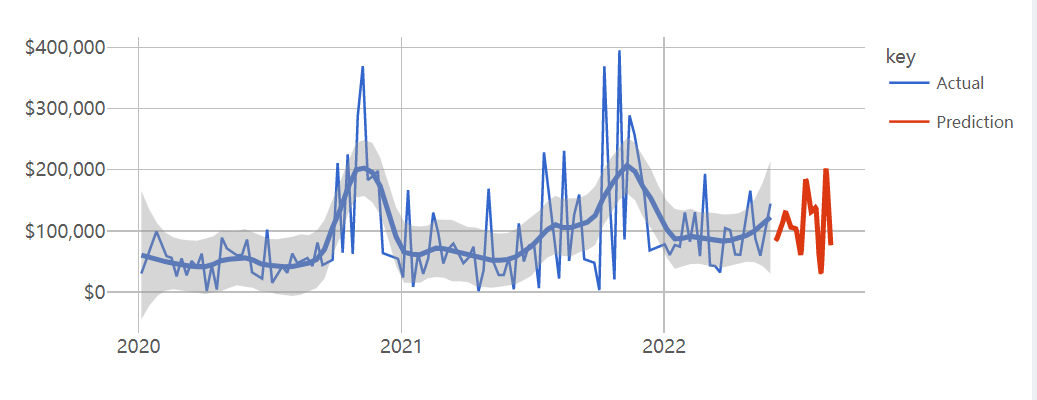
\includegraphics{img/line1.png}

We will create our own R packages \textbf{``Predict Future Order''} to
encapsulate the functions we develop. The given package code contains
four functions that perform different tasks related to time series data
and use it to predict the future order. Here's a description of each
function:

\begin{itemize}
\tightlist
\item
  \textbf{aggregate\_time\_series:} Aggregate\_time\_series: This
  function produces a new time dimension based on dates, such as day,
  week, month, quarter or year, and it calculates the total sales per
  time unit.
\end{itemize}

\begin{Shaded}
\begin{Highlighting}[]
\CommentTok{\#\textquotesingle{} A function that aggregates time series data}
\CommentTok{\#\textquotesingle{}}
\CommentTok{\#\textquotesingle{}This function aggregates the given data based on the specified time unit.}
\CommentTok{\#\textquotesingle{}time\_unit value includes "day", "week", "month", "quarter", "year".}
\CommentTok{\#\textquotesingle{}Then it calculates the total sales for}
\CommentTok{\#\textquotesingle{}each time unit and generates the time series info.}
\CommentTok{\#\textquotesingle{} @author Ting Wei}
\CommentTok{\#\textquotesingle{} @param data A tibble format data, including the following columns:}
\CommentTok{\#\textquotesingle{}   {-} ORDERDATE: A column in POSIXct format,}
\CommentTok{\#\textquotesingle{}   e.g., "2020{-}02{-}24", representing the order dates.}
\CommentTok{\#\textquotesingle{}   {-} SALES: A column recording the sales price.}
\CommentTok{\#\textquotesingle{} @param time\_unit A character string specifying}
\CommentTok{\#\textquotesingle{} the time unit to aggregate the data (default: "month").}
\CommentTok{\#\textquotesingle{} @param ORDERDATE A column in POSIXct format, e.g.,}
\CommentTok{\#\textquotesingle{}  "2020{-}02{-}24", representing the order dates.}
\CommentTok{\#\textquotesingle{} @param SALES A column recording the sales price.}
\CommentTok{\#\textquotesingle{} @return A tibble with the aggregated data,}
\CommentTok{\#\textquotesingle{} including the date and total sales.}
\CommentTok{\#\textquotesingle{} @examples}
\CommentTok{\#\textquotesingle{} \# Example data}
\CommentTok{\#\textquotesingle{} data \textless{}{-} tibble::tribble(}
\CommentTok{\#\textquotesingle{}   \textasciitilde{}ORDERDATE, \textasciitilde{}SALES,}
\CommentTok{\#\textquotesingle{}   "2020{-}02{-}24", 2871,}
\CommentTok{\#\textquotesingle{}   "2020{-}05{-}07", 2766,}
\CommentTok{\#\textquotesingle{}   "2020{-}08{-}30", 3884,}
\CommentTok{\#\textquotesingle{}   \# More rows...}
\CommentTok{\#\textquotesingle{} )}
\CommentTok{\#\textquotesingle{} data$ORDERDATE=as.POSIXct(data$ORDERDATE)}
\CommentTok{\#\textquotesingle{} aggregated\_data \textless{}{-} aggregate\_time\_series(data,}
\CommentTok{\#\textquotesingle{}                                          time\_unit = "month")}
\CommentTok{\#\textquotesingle{} aggregated\_data}
\CommentTok{\#\textquotesingle{} @import dplyr}
\CommentTok{\#\textquotesingle{} @import lubridate}
\CommentTok{\#\textquotesingle{} @import stringr}
\CommentTok{\#\textquotesingle{} @import scales}
\CommentTok{\#\textquotesingle{} @export}

\CommentTok{\#aggregate\_time\_series(processed\_data\_tbl)}
\NormalTok{aggregate\_time\_series }\OtherTok{\textless{}{-}}
  \ControlFlowTok{function}\NormalTok{(data, ORDERDATE,SALES, }\AttributeTok{time\_unit =} \StringTok{"month"}\NormalTok{) \{}

\NormalTok{    output\_tbl }\OtherTok{\textless{}{-}}\NormalTok{ data }\SpecialCharTok{\%\textgreater{}\%}

\NormalTok{      dplyr}\SpecialCharTok{::}\FunctionTok{mutate}\NormalTok{(}\AttributeTok{date =} \FunctionTok{floor\_date}\NormalTok{(ORDERDATE, }\AttributeTok{unit =}\NormalTok{ time\_unit)) }\SpecialCharTok{\%\textgreater{}\%}
      \FunctionTok{group\_by}\NormalTok{(date) }\SpecialCharTok{\%\textgreater{}\%}
      \FunctionTok{summarize}\NormalTok{(}\AttributeTok{total\_sales =} \FunctionTok{sum}\NormalTok{(SALES)) }\SpecialCharTok{\%\textgreater{}\%}
      \FunctionTok{ungroup}\NormalTok{() }\SpecialCharTok{\%\textgreater{}\%}

\NormalTok{      dplyr}\SpecialCharTok{::}\FunctionTok{mutate}\NormalTok{(}\AttributeTok{label\_text =} \FunctionTok{str\_glue}\NormalTok{(}\StringTok{"Date: \{date\}}
\StringTok{                                 Revenue: \{scales::dollar(total\_sales)\}"}\NormalTok{))}
    \FunctionTok{return}\NormalTok{(output\_tbl)}
\NormalTok{  \}}
\end{Highlighting}
\end{Shaded}

\begin{itemize}
\item
  \textbf{plot\_time\_series:} This function plots the time series data,
  showing the total sales over time. It uses the ggplot2 library to
  create a line plot with points, smoothing, and axis labels.
\item
  \textbf{generate\_forecast:} This function generates forecasts for the
  future time periods based on the given time series data. It uses
  different modeling techniques, such as linear regression and XGBoost,
  depending on the time unit of the data. It returns a data frame with
  the actual and predicted values for the time series
\end{itemize}

\begin{Shaded}
\begin{Highlighting}[]
\CommentTok{\#\textquotesingle{} A function that generates forecasts for the time series data}
\CommentTok{\#\textquotesingle{}}
\CommentTok{\#\textquotesingle{} This function generates forecasts for the future}
\CommentTok{\#\textquotesingle{} time periods based on the given data.}
\CommentTok{\#\textquotesingle{}}
\CommentTok{\#\textquotesingle{} @param data A data frame containing the time series data.}
\CommentTok{\#\textquotesingle{} @param n\_future An integer specifying the number}
\CommentTok{\#\textquotesingle{} of future periods to forecast (default: 12 and min:1).}
\CommentTok{\#\textquotesingle{} @param seed An optional seed for reproducibility (default: NULL).}
\CommentTok{\#\textquotesingle{} @return A data frame with the actual}
\CommentTok{\#\textquotesingle{} and predicted values for the time series data.}
\CommentTok{\#\textquotesingle{} @import dplyr}
\CommentTok{\#\textquotesingle{} @import parsnip}
\CommentTok{\#\textquotesingle{} @import tidyverse}
\CommentTok{\#\textquotesingle{} @import stringr}
\CommentTok{\#\textquotesingle{} @import scales}
\CommentTok{\#\textquotesingle{} @import tibble}
\CommentTok{\#\textquotesingle{} @import timetk}
\CommentTok{\#\textquotesingle{} @export}
\NormalTok{generate\_forecast}\OtherTok{=}\ControlFlowTok{function}\NormalTok{(data, }\AttributeTok{n\_future =} \DecValTok{12}\NormalTok{, }\AttributeTok{seed =} \ConstantTok{NULL}\NormalTok{) \{}

\NormalTok{  train\_tbl }\OtherTok{\textless{}{-}}\NormalTok{ data }\SpecialCharTok{\%\textgreater{}\%}
    \FunctionTok{tk\_augment\_timeseries\_signature}\NormalTok{()}

\NormalTok{  future\_data\_tbl }\OtherTok{\textless{}{-}}\NormalTok{ data }\SpecialCharTok{\%\textgreater{}\%}
    \FunctionTok{tk\_index}\NormalTok{() }\SpecialCharTok{\%\textgreater{}\%}
    \FunctionTok{tk\_make\_future\_timeseries}\NormalTok{(}\AttributeTok{n\_future =}\NormalTok{ n\_future, }\AttributeTok{inspect\_weekdays =} \ConstantTok{TRUE}\NormalTok{, }\AttributeTok{inspect\_months =} \ConstantTok{TRUE}\NormalTok{) }\SpecialCharTok{\%\textgreater{}\%}
    \FunctionTok{tk\_get\_timeseries\_signature}\NormalTok{()}

  \CommentTok{\# Isolate and pull scale}
\NormalTok{  time\_scale }\OtherTok{\textless{}{-}}\NormalTok{  data }\SpecialCharTok{\%\textgreater{}\%}
    \FunctionTok{tk\_index}\NormalTok{() }\SpecialCharTok{\%\textgreater{}\%}
    \FunctionTok{tk\_get\_timeseries\_summary}\NormalTok{() }\SpecialCharTok{\%\textgreater{}\%}
    \FunctionTok{pull}\NormalTok{(scale)}

  \CommentTok{\# Linear Regression for "year", XGBoost for other time units}
  \ControlFlowTok{if}\NormalTok{ (time\_scale }\SpecialCharTok{==} \StringTok{"year"}\NormalTok{) \{}
\NormalTok{    model }\OtherTok{\textless{}{-}} \FunctionTok{linear\_reg}\NormalTok{(}\AttributeTok{mode =} \StringTok{"regression"}\NormalTok{) }\SpecialCharTok{\%\textgreater{}\%}
      \FunctionTok{set\_engine}\NormalTok{(}\AttributeTok{engine =} \StringTok{"lm"}\NormalTok{) }\SpecialCharTok{\%\textgreater{}\%}
      \FunctionTok{fit.model\_spec}\NormalTok{(total\_sales }\SpecialCharTok{\textasciitilde{}}\NormalTok{ ., }\AttributeTok{data =}\NormalTok{ train\_tbl }\SpecialCharTok{\%\textgreater{}\%} \FunctionTok{select}\NormalTok{(total\_sales, index.num))}
\NormalTok{  \} }\ControlFlowTok{else}\NormalTok{ \{}
\NormalTok{    seed }\OtherTok{\textless{}{-}}\NormalTok{ seed}
    \FunctionTok{set.seed}\NormalTok{(seed)}
\NormalTok{    model }\OtherTok{\textless{}{-}} \FunctionTok{boost\_tree}\NormalTok{(}
      \AttributeTok{mode =} \StringTok{"regression"}\NormalTok{,}
      \AttributeTok{mtry =} \DecValTok{20}\NormalTok{,}
      \AttributeTok{trees =} \DecValTok{500}\NormalTok{,}
      \AttributeTok{min\_n =} \DecValTok{3}\NormalTok{,}
      \AttributeTok{tree\_depth =} \DecValTok{8}\NormalTok{,}
      \AttributeTok{learn\_rate =} \FloatTok{0.01}\NormalTok{,}
      \AttributeTok{loss\_reduction =} \FloatTok{0.01}\NormalTok{) }\SpecialCharTok{\%\textgreater{}\%}
      \FunctionTok{set\_engine}\NormalTok{(}\AttributeTok{engine =} \StringTok{"xgboost"}\NormalTok{) }\SpecialCharTok{\%\textgreater{}\%}
      \FunctionTok{fit.model\_spec}\NormalTok{(total\_sales }\SpecialCharTok{\textasciitilde{}}\NormalTok{ ., }\AttributeTok{data =}\NormalTok{ train\_tbl }\SpecialCharTok{\%\textgreater{}\%} \FunctionTok{select}\NormalTok{(}\SpecialCharTok{{-}}\NormalTok{date, }\SpecialCharTok{{-}}\NormalTok{label\_text, }\SpecialCharTok{{-}}\NormalTok{diff))}
\NormalTok{  \}}

\NormalTok{  prediction\_tbl }\OtherTok{\textless{}{-}} \FunctionTok{predict}\NormalTok{(model, }\AttributeTok{new\_data =}\NormalTok{ future\_data\_tbl) }\SpecialCharTok{\%\textgreater{}\%}
    \FunctionTok{bind\_cols}\NormalTok{(future\_data\_tbl) }\SpecialCharTok{\%\textgreater{}\%}
    \FunctionTok{select}\NormalTok{(.pred, index) }\SpecialCharTok{\%\textgreater{}\%}
    \FunctionTok{rename}\NormalTok{(}\AttributeTok{total\_sales =}\NormalTok{ .pred,}
           \AttributeTok{date        =}\NormalTok{ index) }\SpecialCharTok{\%\textgreater{}\%}
    \FunctionTok{mutate}\NormalTok{(}\AttributeTok{label\_text =} \FunctionTok{str\_glue}\NormalTok{(}\StringTok{"Date: \{date\}}
\StringTok{                                 Revenue: \{scales::dollar(total\_sales)\}"}\NormalTok{)) }\SpecialCharTok{\%\textgreater{}\%}
    \FunctionTok{add\_column}\NormalTok{(}\AttributeTok{key =} \StringTok{"Prediction"}\NormalTok{)}
\NormalTok{  output\_tbl }\OtherTok{\textless{}{-}}\NormalTok{ data }\SpecialCharTok{\%\textgreater{}\%}
    \FunctionTok{add\_column}\NormalTok{(}\AttributeTok{key =} \StringTok{"Actual"}\NormalTok{) }\SpecialCharTok{\%\textgreater{}\%}
    \FunctionTok{bind\_rows}\NormalTok{(prediction\_tbl)}
  \FunctionTok{return}\NormalTok{(output\_tbl)}
\NormalTok{\}}
\end{Highlighting}
\end{Shaded}

\begin{itemize}
\tightlist
\item
  \textbf{plot\_forecast:} This function plots the actual and predicted
  values for the time series data. It creates a line plot with different
  colored lines for the actual and predicted values. It also includes
  smoothing and point markers for the data points.
\end{itemize}

These functions provide a comprehensive set of tools for aggregating,
visualizing, and forecasting time series data. Presenting
aggregate\_time\_series, and generate\_forecast as example:

\hypertarget{future-order-prediction-table-info}{%
\subsubsection{Future order prediction table
info}\label{future-order-prediction-table-info}}

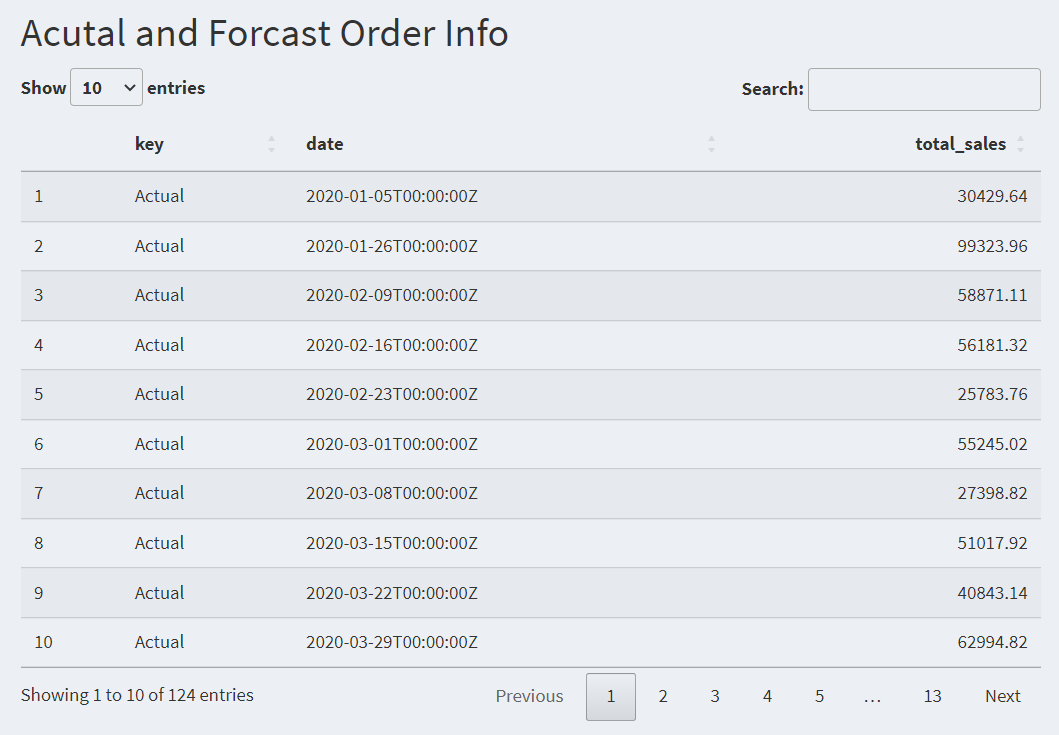
\includegraphics{img/table2.png}

\begin{Shaded}
\begin{Highlighting}[]
\NormalTok{output}\SpecialCharTok{$}\NormalTok{page5\_output02 }\OtherTok{\textless{}{-}}\NormalTok{ DT}\SpecialCharTok{::}\FunctionTok{renderDataTable}\NormalTok{(\{}
  \ControlFlowTok{if}\NormalTok{ (input}\SpecialCharTok{$}\NormalTok{forecast\_mode) \{}
    \FunctionTok{time\_plot\_predictions\_tbl}\NormalTok{()  }\SpecialCharTok{\%\textgreater{}\%}\NormalTok{dplyr}\SpecialCharTok{::}\FunctionTok{select}\NormalTok{(key,date,total\_sales)}
\NormalTok{\}}
  \ControlFlowTok{else}\NormalTok{ \{}\FunctionTok{time\_plot\_tbl}\NormalTok{() }\SpecialCharTok{\%\textgreater{}\%}\NormalTok{dplyr}\SpecialCharTok{::}\FunctionTok{select}\NormalTok{(date,total\_sales)\}}
\NormalTok{\},}\AttributeTok{options =}\NormalTok{ opts)}
\end{Highlighting}
\end{Shaded}

\hypertarget{customer-forcast}{%
\subsection{Customer Forcast}\label{customer-forcast}}

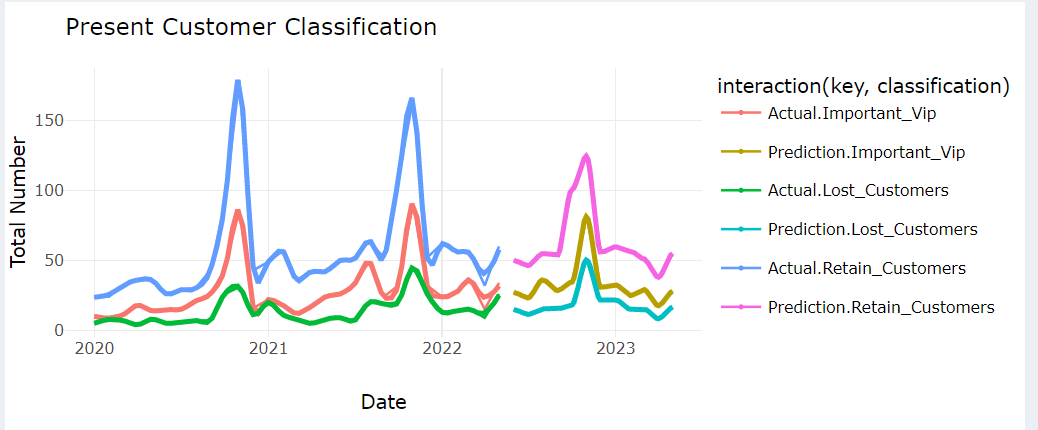
\includegraphics{img/line2.png}

To forecast a customer's future behavior and belonging group. Analyze
the predicted customer behavior to identify segments. Analyzing and
segmenting customers into these categories allows businesses to
prioritize their efforts and allocate resources effectively

\begin{itemize}
\item
  mportant VIP: Important VIP customers are those who hold significant
  value for the business. Identifying and retaining these VIP customers
  is crucial for the success and growth of the business. Companies often
  provide special benefits, personalized services, and exclusive offers
  to maintain a strong relationship with their important VIP customers.
\item
  Lost Customers: Lost customers refer to those who were previously
  engaged with the business but have stopped making purchases or
  interacting with the company. Identifying and understanding the
  reasons for customer churn is essential for businesses to take
  appropriate actions to win back lost customers or prevent further
  customer attrition.
\item
  Retained Customers: Retained customers are the customers who continue
  to engage with the business and make repeat purchases over time.
  Building strong relationships with retained customers through
  personalized communication, rewards programs, and excellent customer
  service is important to maintain their loyalty and maximize their
  lifetime value.
\end{itemize}

\begin{Shaded}
\begin{Highlighting}[]
\NormalTok{customer\_forecast }\OtherTok{\textless{}{-}}
  \ControlFlowTok{function}\NormalTok{(data, }\AttributeTok{n\_future =} \DecValTok{12}\NormalTok{, }\AttributeTok{seed =} \ConstantTok{NULL}\NormalTok{) \{}

\NormalTok{    train\_tbl }\OtherTok{\textless{}{-}}\NormalTok{ data }\SpecialCharTok{\%\textgreater{}\%}
      \FunctionTok{tk\_augment\_timeseries\_signature}\NormalTok{()}

\NormalTok{    future\_data\_tbl }\OtherTok{\textless{}{-}}\NormalTok{ data }\SpecialCharTok{\%\textgreater{}\%}
      \FunctionTok{tk\_index}\NormalTok{() }\SpecialCharTok{\%\textgreater{}\%}\FunctionTok{unique}\NormalTok{()}\SpecialCharTok{\%\textgreater{}\%}
      \FunctionTok{tk\_make\_future\_timeseries}\NormalTok{(}\AttributeTok{n\_future =}\NormalTok{ n\_future,}
                                \AttributeTok{inspect\_weekdays =} \ConstantTok{TRUE}\NormalTok{,}
                                \AttributeTok{inspect\_months =} \ConstantTok{TRUE}\NormalTok{) }\SpecialCharTok{\%\textgreater{}\%}
      \FunctionTok{tk\_get\_timeseries\_signature}\NormalTok{()}

\NormalTok{    future\_data\_tbl}\OtherTok{\textless{}{-}}\NormalTok{ future\_data\_tbl[}\FunctionTok{rep}\NormalTok{(}\FunctionTok{row.names}\NormalTok{(future\_data\_tbl),}
                                          \AttributeTok{each =} \DecValTok{3}\NormalTok{), ]}

\NormalTok{    categories }\OtherTok{\textless{}{-}} \FunctionTok{c}\NormalTok{(}\StringTok{"Retain\_Customers"}\NormalTok{,}
                    \StringTok{"Lost\_Customers"}\NormalTok{, }\StringTok{"Important\_Vip"}\NormalTok{)}
\NormalTok{    num\_rows }\OtherTok{\textless{}{-}} \FunctionTok{nrow}\NormalTok{(future\_data\_tbl)}
\NormalTok{    repeated\_categories }\OtherTok{\textless{}{-}} \FunctionTok{rep}\NormalTok{(categories, }\AttributeTok{length.out =}\NormalTok{ num\_rows)}
\NormalTok{    future\_data\_tbl}\SpecialCharTok{$}\NormalTok{classification }\OtherTok{\textless{}{-}}\NormalTok{ repeated\_categories}

    \CommentTok{\# Isolate and pull scale}
\NormalTok{    time\_scale }\OtherTok{\textless{}{-}}\NormalTok{  data }\SpecialCharTok{\%\textgreater{}\%}
      \FunctionTok{tk\_index}\NormalTok{() }\SpecialCharTok{\%\textgreater{}\%}\FunctionTok{unique}\NormalTok{()}\SpecialCharTok{\%\textgreater{}\%}
      \FunctionTok{tk\_get\_timeseries\_summary}\NormalTok{() }\SpecialCharTok{\%\textgreater{}\%}
      \FunctionTok{pull}\NormalTok{(scale)}

    \CommentTok{\# Linear Regression for "year", XGBoost for other time units}
    \ControlFlowTok{if}\NormalTok{ (time\_scale }\SpecialCharTok{==} \StringTok{"year"}\NormalTok{) \{}
\NormalTok{      model }\OtherTok{\textless{}{-}} \FunctionTok{linear\_reg}\NormalTok{(}\AttributeTok{mode =} \StringTok{"regression"}\NormalTok{) }\SpecialCharTok{\%\textgreater{}\%}
        \FunctionTok{set\_engine}\NormalTok{(}\AttributeTok{engine =} \StringTok{"lm"}\NormalTok{) }\SpecialCharTok{\%\textgreater{}\%}
        \FunctionTok{fit.model\_spec}\NormalTok{(total\_num }\SpecialCharTok{\textasciitilde{}}\NormalTok{ .,}
                       \AttributeTok{data =}\NormalTok{ train\_tbl }\SpecialCharTok{\%\textgreater{}\%}
                         \FunctionTok{select}\NormalTok{(total\_num,classification ,index.num))}
\NormalTok{    \} }\ControlFlowTok{else}\NormalTok{ \{}
\NormalTok{      seed }\OtherTok{\textless{}{-}}\NormalTok{ seed}
      \FunctionTok{set.seed}\NormalTok{(seed)}
\NormalTok{      model }\OtherTok{\textless{}{-}} \FunctionTok{boost\_tree}\NormalTok{(}
        \AttributeTok{mode =} \StringTok{"regression"}\NormalTok{,}
        \AttributeTok{mtry =} \DecValTok{20}\NormalTok{,}
        \AttributeTok{trees =} \DecValTok{500}\NormalTok{,}
        \AttributeTok{min\_n =} \DecValTok{3}\NormalTok{,}
        \AttributeTok{tree\_depth =} \DecValTok{8}\NormalTok{,}
        \AttributeTok{learn\_rate =} \FloatTok{0.01}\NormalTok{,}
        \AttributeTok{loss\_reduction =} \FloatTok{0.01}\NormalTok{) }\SpecialCharTok{\%\textgreater{}\%}
        \FunctionTok{set\_engine}\NormalTok{(}\AttributeTok{engine =} \StringTok{"xgboost"}\NormalTok{) }\SpecialCharTok{\%\textgreater{}\%}
        \FunctionTok{fit.model\_spec}\NormalTok{(total\_num }\SpecialCharTok{\textasciitilde{}}\NormalTok{ .,}
                       \AttributeTok{data =}\NormalTok{ train\_tbl }\SpecialCharTok{\%\textgreater{}\%} \FunctionTok{select}\NormalTok{(}\SpecialCharTok{{-}}\NormalTok{date,  }\SpecialCharTok{{-}}\NormalTok{diff))}

\NormalTok{    \}}
\end{Highlighting}
\end{Shaded}




\end{document}
